\documentclass[review]{elsarticle}

\graphicspath{{./figures/}}

\usepackage{graphicx}
\usepackage{hyperref}
\usepackage{float}
\usepackage{verbatim}
\usepackage{apalike}
\usepackage{amsmath}
\usepackage{amssymb}
\usepackage{booktabs}
\usepackage{multirow}
\usepackage{subcaption}

\restylefloat{figure}
\floatstyle{plaintop}
\restylefloat{table}

\journal{Expert Systems with Applications}

\begin{document}

\begin{frontmatter}

% =========================================================
% TITLE PAGE
% =========================================================

\begin{titlepage}
\begin{center}

\vspace*{1cm}

\textbf{\large COS 791 Image Analysis and Understanding: Multilevel Thresholding}

\vspace{1.5cm}

% Replace author details with your actual group members.
Aryan Mohanlall$^{a}$ (u23565536@tuks.co.za),
Zingisa Matwana$^{a}$ (u25719302@tuks.co.za),
Third Author$^{a}$ (third.author@mail.com),
Fourth Author$^{a}$ (fourth.author@mail.com) \\

\vspace{0.5cm}

\begin{flushleft}
\small
$^a$ Department of Computer Science, University of Pretoria,
Pretoria, Gauteng, South Africa

\vspace{1cm}

\textbf{Corresponding author:} Aryan Mohanlall \\
Department of Computer Science, University of Pretoria \\
Pretoria, Gauteng, South Africa \\
Email: u23565536@tuks.co.za

\end{flushleft}

\end{center}
\end{titlepage}


% =========================================================
% ARTICLE INFORMATION
% =========================================================

\title{Differential Evolution for Multilevel Image Thresholding Using Otsu, Kapur and Tsallis Objective Functions}

\author[label1]{Aryan Mohanlall \corref{cor1}}
\ead{u23565536@tuks.co.za}

\author[label1]{Zingisa Matwana}
\ead{u25719302@tuks.co.za}

\author[label1]{Third Author}
\ead{third.author@mail.com}

\author[label1]{Fourth Author}
\ead{fourth.author@mail.com}

\cortext[cor1]{Corresponding author.}

\address[label1]
{Department of Computer Science, University of Pretoria,
Pretoria, Gauteng, South Africa}


% =========================================================
% ABSTRACT
% =========================================================

\begin{abstract}

Multilevel image thresholding is an unsupervised image segmentation
technique in which multiple intensity thresholds are selected to divide
an image into homogeneous regions. As the number of thresholds increases,
exhaustive threshold optimisation becomes computationally expensive,
motivating the use of population-based optimisation algorithms.

This study investigates the application of five Differential Evolution
(DE) variants---Standard DE, JADE, SHADE, L-SHADE, and Late Acceptance
Differential Evolution (LADE)---to multilevel image thresholding.
Three optimisation objectives are considered: Otsu's between-class
variance, Kapur's entropy, and Tsallis non-extensive entropy.

The algorithms are evaluated at threshold levels
$K \in \{3,5,7,9,11,12\}$ using standard BSD500 images and CHAOS
magnetic resonance imaging (MRI) scans. Performance is evaluated using
image reconstruction quality, segmentation quality, convergence
behaviour, statistical significance, and computational scalability.

% ---------------------------------------------------------
% COMPLETE AFTER EXPERIMENTS:
% Add 2--4 sentences summarising your most important numerical results.
%
% Example structure:
%
% Results indicate that [algorithm] achieved the highest average
% [metric] for [dataset/objective/K], while [algorithm] demonstrated
% [convergence/scalability observation].
%
% Statistical analysis showed ...
% ---------------------------------------------------------

The findings provide an empirical comparison of adaptive and
non-adaptive Differential Evolution approaches for increasingly
high-dimensional multilevel threshold selection.

\end{abstract}


\begin{keyword}
Multilevel thresholding
\sep Differential Evolution
\sep JADE
\sep SHADE
\sep L-SHADE
\sep Late Acceptance
\sep Otsu
\sep Kapur entropy
\sep Tsallis entropy
\sep Image segmentation
\end{keyword}

\end{frontmatter}


% =========================================================
% 1. INTRODUCTION
% =========================================================

\section{Introduction}
\label{sec:introduction}

Image segmentation is the process of partitioning an image into
meaningful regions and constitutes an important preprocessing step in
many computer vision and medical image analysis applications.

Thresholding represents one of the simplest forms of image segmentation.
In binary thresholding, a single threshold separates pixels into two
classes. Multilevel thresholding generalises this concept by introducing
multiple thresholds, allowing an image to be partitioned into several
intensity regions.

For an image containing $L$ possible grey levels, selecting an optimal
combination of $K$ thresholds becomes increasingly computationally
expensive as $K$ increases. Consequently, exhaustive search becomes
impractical for high-dimensional multilevel thresholding problems.
Metaheuristic optimisation techniques provide an alternative mechanism
for searching this threshold space.

Differential Evolution (DE) is a population-based evolutionary
optimisation algorithm based on mutation, crossover, and selection.
Several adaptive DE variants have subsequently been developed to improve
parameter adaptation, convergence behaviour, population diversity, and
computational efficiency.

This study compares five DE-based optimisation algorithms for multilevel
image thresholding:

\begin{enumerate}
    \item Standard Differential Evolution (DE/rand/1/bin);
    \item JADE;
    \item SHADE;
    \item L-SHADE; and
    \item Late Acceptance Differential Evolution (LADE).
\end{enumerate}

The algorithms are used to optimise three thresholding criteria:
Otsu's between-class variance, Kapur's information entropy, and
Tsallis non-extensive entropy.

The experiments are conducted in two phases. The first evaluates
algorithm behaviour on standard BSD500 benchmark images, while the
second investigates performance on CHAOS MRI medical images.

The main objectives of this study are therefore to:

\begin{itemize}
    \item implement and compare five Differential Evolution variants;
    \item evaluate Otsu, Kapur, and Tsallis optimisation objectives;
    \item investigate performance as the number of thresholds increases;
    \item evaluate image reconstruction and segmentation quality;
    \item compare convergence behaviour between algorithms;
    \item evaluate computational scalability with increasing $K$; and
    \item determine whether observed algorithmic differences are
          statistically significant.
\end{itemize}


% =========================================================
% 2. BACKGROUND AND RELATED WORK
% =========================================================

\section{Background and Related Work}
\label{sec:background}

% This section is where most of your literature citations should go.

\subsection{Multilevel Image Thresholding}

Consider a grey-scale image $I$ of size $M \times N$ with
$L$ possible intensity levels

\begin{equation}
\{0,1,\ldots,L-1\}.
\end{equation}

The normalised probability of intensity level $i$ is

\begin{equation}
p_i =
\frac{h(i)}{M N},
\end{equation}

where $h(i)$ represents the number of pixels with intensity $i$.

For $K$ thresholds,

\begin{equation}
\mathbf{t} =
[t_1,t_2,\ldots,t_K],
\end{equation}

the thresholds must satisfy

\begin{equation}
0 < t_1 < t_2 < \cdots < t_K < L-1.
\end{equation}

These thresholds partition the image into $K+1$ intensity classes,

\begin{equation}
C_0,C_1,\ldots,C_K.
\end{equation}


\subsection{Otsu's Between-Class Variance}
\label{sec:otsu}

% Explain Otsu based on the literature.
% Add the exact equations used by your implementation.
%
% Explain:
% - class probabilities
% - class means
% - global mean
% - between-class variance
% - maximisation objective

Otsu's method selects thresholds by maximising the between-class
variance of the resulting intensity classes.

% TODO: Insert complete Otsu multilevel formulation and citation.


\subsection{Kapur's Information Entropy}
\label{sec:kapur}

Kapur's method formulates threshold selection as an entropy maximisation
problem.

% TODO:
% - Define entropy for each intensity class.
% - Define total entropy.
% - Explain why larger entropy is preferred.
% - Cite original/relevant literature.


\subsection{Tsallis Non-Extensive Entropy}
\label{sec:tsallis}

Tsallis entropy generalises conventional information entropy through
the introduction of the non-extensivity parameter $q$.

% TODO:
% Insert actual equation used by your implementation.
%
% Explicitly explain:
% q = 1 relationship to conventional entropy
% selected q value(s), e.g. q = 0.8
% why q changes the optimisation landscape


\subsection{Differential Evolution}
\label{sec:de_background}

Differential Evolution is a stochastic population-based optimisation
algorithm operating through mutation, crossover, and selection.

% Explain generic DE before discussing variants.

\subsubsection{Mutation}

For the DE/rand/1 strategy,

\begin{equation}
\mathbf{v}_{i}
=
\mathbf{x}_{r_1}
+
F
\left(
\mathbf{x}_{r_2}
-
\mathbf{x}_{r_3}
\right),
\end{equation}

where $r_1$, $r_2$, and $r_3$ are mutually distinct randomly selected
population indices and $F$ is the differential weight.


\subsubsection{Binomial Crossover}

The trial vector is generated according to

\begin{equation}
u_{i,j}
=
\begin{cases}
v_{i,j},
& \text{if } rand_j \leq CR
\text{ or } j=j_{\mathrm{rand}}, \\

x_{i,j},
& \text{otherwise}.
\end{cases}
\end{equation}


\subsubsection{Selection}

For a maximisation problem,

\begin{equation}
\mathbf{x}_{i}^{(g+1)}
=
\begin{cases}
\mathbf{u}_{i},
& f(\mathbf{u}_{i}) \geq f(\mathbf{x}_{i}),\\

\mathbf{x}_{i},
& \text{otherwise}.
\end{cases}
\end{equation}


% =========================================================
% 3. PROPOSED / IMPLEMENTED ALGORITHMS
% =========================================================

\section{Differential Evolution Algorithms}
\label{sec:algorithms}


\subsection{Standard Differential Evolution}

The baseline algorithm uses the DE/rand/1/bin strategy.

% TODO:
% Specify:
% - population size
% - F
% - CR
% - boundary handling
% - integer threshold conversion
% - duplicate threshold handling
% - sorting of thresholds


\subsection{JADE}
\label{sec:jade}

JADE follows the adaptive DE/current-to-$p$best/1 mechanism introduced by Zhang and Sanderson \citep{zhang2009jade}. In the original JADE formulation, the mutant vector for target $\mathbf{x}_{i,g}$ is
\begin{equation}
\mathbf{v}_{i,g}
=
\mathbf{x}_{i,g}
+ F_i(\mathbf{x}_{pbest,g}-\mathbf{x}_{i,g})
+ F_i(\mathbf{x}_{r_1,g}-\mathbf{x}_{r_2,g}).
\end{equation}
For this project, the same current-to-$p$best/1 strategy is used, but the vectors are threshold candidates rather than unconstrained real-valued design variables. The index $pbest$ is sampled uniformly from the top $\lceil p N_P \rceil$ parent candidates, where $p=0.05$ and $N_P=50$ in the JADE runs. The index $r_1$ is selected from the current parent population, excluding the target. The second donor index $r_2$ is selected uniformly from the union of the parent population and the external archive, excluding the target and the $r_1$ population index. This distinction matters because the original JADE algorithm is adaptive and archive-based, whereas the project-specific threshold representation is handled separately by the shared segmentation decoder and clipping rules.

Within each generation, the parent population and the corresponding fitness values are frozen before mutation and trial evaluation. Accepted offspring are stored in a separate next-generation population and are committed only at the end of the generation; this also applies to the final partial generation when the evaluation budget is exhausted. The archive stores displaced parents immediately after a strict improvement, and, if the archive exceeds $N_P$ entries at generation end, it is randomly trimmed back to a maximum of $N_P$ solutions. This is consistent with the project implementation used here and differs from an in-place update strategy that would overwrite parents during the generation.

Binomial crossover is then applied to each target vector with a mandatory mutant component, ensuring that at least one dimension is inherited from the mutant. The objective functions are maximised, so only strictly higher fitness values are accepted; equal or lower fitness values do not replace the parent. Control parameters are sampled as in JADE: $CR_i \sim \mathcal{N}(\mu_{CR}, 0.1)$, clipped to $[0,1]$, and $F_i \sim \mathcal{C}(\mu_F, 0.1)$ with non-positive or non-finite values resampled and values above one capped at one. The successful parameter sets update the adaptation means as
\begin{align}
\mu_{CR} &\leftarrow
(1-c)\mu_{CR}+c\,\operatorname{mean}(S_{CR}),\\
\mu_F &\leftarrow
(1-c)\mu_F+
 c\,\frac{\sum_{F\in S_F}F^2}{\sum_{F\in S_F}F},
\end{align}
where the second update is the Lehmer mean of successful mutation factors. If no successful trial is found in a generation, the means remain unchanged.

After mutation and crossover, each real-valued threshold vector is transformed to an integer threshold set using the shared implementation in \texttt{src/segmentation.py}. The project decoder rounds to the nearest integer, clips every threshold into the valid range $[1,254]$, and then enforces a strictly increasing set of threshold values by pushing each component upward to at least the lower bound for that position and pushing it downward to respect the upper bound implied by later thresholds. This yields valid, ordered integer thresholds that conform to the project segmentation code and are not equivalent to unconstrained mutation in the original JADE paper. Mutants that fall outside the threshold bounds are clipped before decoding, and the final integer threshold vector is used in the objective evaluation.

The FE budget follows the project implementation exactly: the initial population evaluation consumes $N_P$ evaluations, and every evaluated trial thereafter increments the objective budget. The optimiser stops once the budget is reached, including the final partial generation when a generation is terminated by the evaluation cap. The total experimental configuration for JADE is $N_P=50$, $p=0.05$, $c=0.1$, initial $\mu_F=\mu_{CR}=0.5$, archive enabled with capacity 50, bounds $[1,254]$, 30 independent runs, 30,000 function evaluations including initialisation, and four workers.

\subsection{SHADE}

SHADE uses success-history based adaptation to maintain historical
memories of successful $F$ and $CR$ parameter values.

% TODO:
% Explain:
% - memory M_F
% - memory M_CR
% - success history
% - sampling F and CR
% - memory update mechanism


\subsection{L-SHADE}

L-SHADE extends SHADE through Linear Population Size Reduction (LPSR).

% TODO:
% Explain:
% - how population size decreases
% - initial population size
% - minimum population size
% - relationship to consumed FEs


\subsection{Late Acceptance Differential Evolution}

LADE integrates a Late Acceptance mechanism into Differential Evolution.

% TODO:
% This section MUST match your actual implementation.
%
% Explain:
% - late acceptance history/list
% - acceptance condition
% - history length
% - how the mechanism changes ordinary DE selection
% - mutation/crossover strategy used


% =========================================================
% 4. METHODOLOGY
% =========================================================

\section{Methodology}
\label{sec:methodology}


\subsection{Threshold Representation}

Each candidate solution consists of $K$ threshold values:

\begin{equation}
\mathbf{x}_i =
[t_1,t_2,\ldots,t_K].
\end{equation}

Since pixel intensities are discrete, candidate threshold values produced
by Differential Evolution must ultimately be mapped to valid integer
intensities.

% TODO:
% Explain precisely how your code:
% - rounds/clips values
% - sorts thresholds
% - handles duplicates
% - guarantees 0 < t1 < ... < tK < 255


\subsection{Threshold Levels}

The following numbers of thresholds are evaluated:

\begin{equation}
K \in \{3,5,7,9,11,12\}.
\end{equation}


\subsection{Datasets}


\subsubsection{BSD500 Benchmark Dataset}

The first experimental phase uses 10 standard test images from the
BSD500 dataset.

% TODO:
% - identify the exact 10 images
% - image dimensions if relevant
% - grayscale conversion
% - preprocessing performed
% - why these images were selected


\subsubsection{CHAOS MRI Dataset}

The second experimental phase evaluates the optimisation algorithms on
15 MRI scan images from the CHAOS dataset.

% TODO:
% - modality used
% - exact images/slices
% - preprocessing
% - normalisation
% - ground-truth masks
% - GT mask matching procedure


\subsection{Experimental Parameters}

Table~\ref{tab:parameters} summarises the main experimental settings.

\begin{table}[H]
\caption{Experimental parameter settings.}
\label{tab:parameters}
\centering

\begin{tabular}{ll}
\toprule
\textbf{Parameter} & \textbf{Setting} \\
\midrule

Algorithms &
DE, JADE, SHADE, L-SHADE, LADE \\

Objective functions &
Otsu, Kapur, Tsallis \\

Threshold levels &
$3,5,7,9,11,12$ \\

Independent runs &
30 \\

JADE population size &
50 \\

JADE $p$ &
0.05 (three p-best candidates) \\

JADE adaptation rate $c$ &
0.1 \\

JADE initial $\mu_F$, $\mu_{CR}$ &
0.5, 0.5 \\

JADE sampling scale for $F$ &
0.1 (Cauchy distribution) \\

JADE sampling standard deviation for $CR$ &
0.1 (normal distribution) \\

JADE external archive &
Enabled; maximum 50 solutions \\

JADE threshold bounds &
$[1,254]$ \\

JADE mutant boundary handling &
Clipping \\

JADE initialisation evaluations &
50, included in the total budget \\

Maximum function evaluations &
30,000 per run, including initialisation \\

Tsallis $q$ &
0.8 \\

Parallel workers for JADE experiments &
4 \\

Independent random seeds &
Deterministic seeds derived from each task and run \\

\bottomrule
\end{tabular}

For the JADE experiments, random seeds were generated
deterministically using an eight-byte BLAKE2b digest of
the base seed, image identifier, objective, threshold count
and run index, reduced modulo $2^{32}$. The base seed was
\texttt{0xC05791}. Initial population evaluation consumed
50 of the 30,000 objective-function evaluations permitted
per run.

\end{table}


\subsection{Experimental Procedure}

For every image, objective function, threshold level and optimisation
algorithm, 30 independent optimisation runs are performed.

Each algorithm receives the same maximum number of objective function
evaluations to ensure that algorithms are compared under an equivalent
computational optimisation budget.

For each independent run, the following information is recorded:

\begin{itemize}
    \item best objective-function value;
    \item optimal threshold vector;
    \item PSNR;
    \item SSIM;
    \item uniformity;
    \item execution time;
    \item function evaluations; and
    \item convergence history.
\end{itemize}


% =========================================================
% 5. EVALUATION METRICS
% =========================================================

\section{Evaluation Metrics}
\label{sec:metrics}


\subsection{Peak Signal-to-Noise Ratio}

The Peak Signal-to-Noise Ratio (PSNR) is calculated from the mean
squared error (MSE),

\begin{equation}
MSE =
\frac{1}{MN}
\sum_{i=1}^{M}
\sum_{j=1}^{N}
\left(
I(i,j)-\hat{I}(i,j)
\right)^2.
\end{equation}

PSNR is then defined as

\begin{equation}
PSNR =
10\log_{10}
\left(
\frac{MAX_I^2}{MSE}
\right).
\end{equation}

% Explain what higher/lower means.


\subsection{Structural Similarity Index}

The Structural Similarity Index (SSIM) measures structural similarity
between the original image and its reconstructed or segmented
representation.

% TODO:
% Add SSIM formulation or cite implementation.
% Explain interpretation.


\subsection{Feature Uniformity}

% IMPORTANT:
% Use the exact uniformity equation required by your implementation/
% literature source.

The uniformity metric measures the homogeneity of pixels contained
within the regions produced by multilevel thresholding.

% TODO: Insert equation.


\subsection{Dice Similarity Coefficient}

For the CHAOS experiment, the Dice coefficient is defined as

\begin{equation}
Dice =
\frac{2|A \cap B|}
{|A|+|B|},
\end{equation}

where $A$ represents the predicted segmentation and $B$ represents the
ground-truth mask.

\subsection{Jaccard Index}

The Jaccard index is defined as

\begin{equation}
J(A,B)
=
\frac{|A\cap B|}
{|A\cup B|}.
\end{equation}


\subsection{Execution Time}

Execution time is measured to investigate the computational cost of
each optimisation algorithm as dimensionality increases.

% State:
% - units
% - timing function
% - whether preprocessing is included
% - machine specification


% =========================================================
% 6. EXPERIMENT 1 -- BSD500
% =========================================================
 
\section{Experiment 1: BSD500 Benchmark Images}

\label{sec:experiment1}

\subsection{Experimental Objective and Completed Runs}

This section reports the completed Standard DE (DE), Late Acceptance DE (LADE) and JADE experiments on the ten supplied BSD500 images. Results for SHADE and L-SHADE are not included in this comparison. Each algorithm was evaluated with Otsu, Kapur and Tsallis ($q=0.8$) at $K\in\{3,5,7,9,11,12\}$, using 30 runs per combination and a budget of 30,000 function evaluations, including initialisation. The saved results contain 5,400 successful runs per algorithm (16,200 in total); every run used the full budget and passed the recorded fitness-contract check.

\subsection{Reconstruction Performance}

Tables below report the mean and sample standard deviation of PSNR, SSIM and uniformity. Each entry pools 300 observations: 30 independent runs on each of ten images. Consequently, these standard deviations combine differences between images with stochastic variation within an image; they should not be interpreted solely as algorithm stability. Per-image means and standard deviations over the 30 runs are supplied in \texttt{report/exp1\_per\_image\_summary.csv}. Metrics use class-mean reconstruction, and higher values indicate better reconstruction quality. The displayed values are descriptive comparisons, without a claim of statistical significance.

\begin{table}[htbp]
\centering
\small
\caption{PSNR (dB) on BSD500 using Otsu: pooled mean $\pm$ sample standard deviation across 300 observations per entry (10 images, 30 runs each).}
\label{tab:bsd-otsu-psnr}
\resizebox{\textwidth}{!}{%
\begin{tabular}{lcccccc}
\toprule
Algorithm & $K=3$ & $K=5$ & $K=7$ & $K=9$ & $K=11$ & $K=12$ \\
\midrule
DE & $24.5370 \pm 1.1806$ & $28.3282 \pm 1.1253$ & $30.8671 \pm 1.1393$ & $32.4792 \pm 1.2043$ & $33.7545 \pm 1.2723$ & $34.3369 \pm 1.2678$ \\
LADE & $24.5370 \pm 1.1806$ & $28.3282 \pm 1.1253$ & $30.7982 \pm 1.1365$ & $32.4163 \pm 1.2276$ & $33.7414 \pm 1.2606$ & $34.2962 \pm 1.2471$ \\
JADE & $24.5370 \pm 1.1806$ & $28.3282 \pm 1.1253$ & $30.9290 \pm 1.1367$ & $32.9960 \pm 1.2018$ & $34.6155 \pm 1.2258$ & $35.3331 \pm 1.2486$ \\
\bottomrule
\end{tabular}%
}
\end{table}

\begin{table}[htbp]
\centering
\small
\caption{SSIM on BSD500 using Otsu: pooled mean $\pm$ sample standard deviation across 300 observations per entry (10 images, 30 runs each).}
\label{tab:bsd-otsu-ssim}
\resizebox{\textwidth}{!}{%
\begin{tabular}{lcccccc}
\toprule
Algorithm & $K=3$ & $K=5$ & $K=7$ & $K=9$ & $K=11$ & $K=12$ \\
\midrule
DE & $0.7419 \pm 0.0347$ & $0.8371 \pm 0.0296$ & $0.8841 \pm 0.0180$ & $0.9091 \pm 0.0162$ & $0.9256 \pm 0.0142$ & $0.9328 \pm 0.0130$ \\
LADE & $0.7419 \pm 0.0347$ & $0.8371 \pm 0.0296$ & $0.8828 \pm 0.0184$ & $0.9086 \pm 0.0162$ & $0.9260 \pm 0.0140$ & $0.9323 \pm 0.0127$ \\
JADE & $0.7419 \pm 0.0347$ & $0.8371 \pm 0.0296$ & $0.8847 \pm 0.0180$ & $0.9147 \pm 0.0149$ & $0.9341 \pm 0.0132$ & $0.9414 \pm 0.0115$ \\
\bottomrule
\end{tabular}%
}
\end{table}

\begin{table}[htbp]
\centering
\small
\caption{Uniformity on BSD500 using Otsu: pooled mean $\pm$ sample standard deviation across 300 observations per entry (10 images, 30 runs each).}
\label{tab:bsd-otsu-uniformity}
\resizebox{\textwidth}{!}{%
\begin{tabular}{lcccccc}
\toprule
Algorithm & $K=3$ & $K=5$ & $K=7$ & $K=9$ & $K=11$ & $K=12$ \\
\midrule
DE & $0.9774 \pm 0.0050$ & $0.9843 \pm 0.0032$ & $0.9878 \pm 0.0025$ & $0.9891 \pm 0.0024$ & $0.9900 \pm 0.0023$ & $0.9905 \pm 0.0022$ \\
LADE & $0.9774 \pm 0.0050$ & $0.9843 \pm 0.0032$ & $0.9876 \pm 0.0026$ & $0.9889 \pm 0.0025$ & $0.9900 \pm 0.0023$ & $0.9904 \pm 0.0022$ \\
JADE & $0.9774 \pm 0.0050$ & $0.9843 \pm 0.0032$ & $0.9880 \pm 0.0025$ & $0.9903 \pm 0.0021$ & $0.9919 \pm 0.0018$ & $0.9925 \pm 0.0017$ \\
\bottomrule
\end{tabular}%
}
\end{table}

\begin{table}[htbp]
\centering
\small
\caption{PSNR (dB) on BSD500 using Kapur: pooled mean $\pm$ sample standard deviation across 300 observations per entry (10 images, 30 runs each).}
\label{tab:bsd-kapur-psnr}
\resizebox{\textwidth}{!}{%
\begin{tabular}{lcccccc}
\toprule
Algorithm & $K=3$ & $K=5$ & $K=7$ & $K=9$ & $K=11$ & $K=12$ \\
\midrule
DE & $19.4855 \pm 1.6350$ & $22.4685 \pm 2.4731$ & $25.6184 \pm 3.4754$ & $28.8529 \pm 3.7906$ & $30.2395 \pm 3.8729$ & $30.9094 \pm 4.0271$ \\
LADE & $19.4829 \pm 1.6353$ & $22.4801 \pm 2.4816$ & $25.5455 \pm 3.4747$ & $28.9409 \pm 3.7814$ & $30.2923 \pm 3.9450$ & $31.1000 \pm 3.8924$ \\
JADE & $19.4827 \pm 1.6354$ & $22.4220 \pm 2.4380$ & $25.3850 \pm 3.3018$ & $28.6743 \pm 3.8546$ & $30.8945 \pm 4.2187$ & $31.9440 \pm 4.2093$ \\
\bottomrule
\end{tabular}%
}
\end{table}

\begin{table}[htbp]
\centering
\small
\caption{SSIM on BSD500 using Kapur: pooled mean $\pm$ sample standard deviation across 300 observations per entry (10 images, 30 runs each).}
\label{tab:bsd-kapur-ssim}
\resizebox{\textwidth}{!}{%
\begin{tabular}{lcccccc}
\toprule
Algorithm & $K=3$ & $K=5$ & $K=7$ & $K=9$ & $K=11$ & $K=12$ \\
\midrule
DE & $0.7331 \pm 0.0455$ & $0.8077 \pm 0.0335$ & $0.8472 \pm 0.0330$ & $0.8696 \pm 0.0278$ & $0.8882 \pm 0.0283$ & $0.8986 \pm 0.0281$ \\
LADE & $0.7330 \pm 0.0455$ & $0.8081 \pm 0.0336$ & $0.8462 \pm 0.0299$ & $0.8702 \pm 0.0283$ & $0.8894 \pm 0.0296$ & $0.8994 \pm 0.0279$ \\
JADE & $0.7330 \pm 0.0455$ & $0.8054 \pm 0.0321$ & $0.8496 \pm 0.0326$ & $0.8756 \pm 0.0253$ & $0.8961 \pm 0.0287$ & $0.9072 \pm 0.0283$ \\
\bottomrule
\end{tabular}%
}
\end{table}

\begin{table}[htbp]
\centering
\small
\caption{Uniformity on BSD500 using Kapur: pooled mean $\pm$ sample standard deviation across 300 observations per entry (10 images, 30 runs each).}
\label{tab:bsd-kapur-uniformity}
\resizebox{\textwidth}{!}{%
\begin{tabular}{lcccccc}
\toprule
Algorithm & $K=3$ & $K=5$ & $K=7$ & $K=9$ & $K=11$ & $K=12$ \\
\midrule
DE & $0.9245 \pm 0.0299$ & $0.9315 \pm 0.0390$ & $0.9444 \pm 0.0532$ & $0.9576 \pm 0.0643$ & $0.9592 \pm 0.0700$ & $0.9587 \pm 0.0769$ \\
LADE & $0.9244 \pm 0.0299$ & $0.9316 \pm 0.0390$ & $0.9436 \pm 0.0542$ & $0.9585 \pm 0.0631$ & $0.9584 \pm 0.0737$ & $0.9612 \pm 0.0737$ \\
JADE & $0.9244 \pm 0.0299$ & $0.9310 \pm 0.0387$ & $0.9426 \pm 0.0527$ & $0.9569 \pm 0.0611$ & $0.9599 \pm 0.0744$ & $0.9621 \pm 0.0786$ \\
\bottomrule
\end{tabular}%
}
\end{table}

\begin{table}[htbp]
\centering
\small
\caption{PSNR (dB) on BSD500 using Tsallis ($q=0.8$): pooled mean $\pm$ sample standard deviation across 300 observations per entry (10 images, 30 runs each).}
\label{tab:bsd-tsallis-psnr}
\resizebox{\textwidth}{!}{%
\begin{tabular}{lcccccc}
\toprule
Algorithm & $K=3$ & $K=5$ & $K=7$ & $K=9$ & $K=11$ & $K=12$ \\
\midrule
DE & $19.9679 \pm 1.5122$ & $22.2757 \pm 1.9052$ & $24.9285 \pm 2.7596$ & $26.7242 \pm 3.1667$ & $27.9688 \pm 3.4248$ & $28.5999 \pm 3.5581$ \\
LADE & $19.9686 \pm 1.5106$ & $22.2775 \pm 1.9060$ & $24.8655 \pm 2.7263$ & $26.8159 \pm 3.2056$ & $27.9820 \pm 3.4180$ & $28.6270 \pm 3.6095$ \\
JADE & $19.9686 \pm 1.5106$ & $22.2741 \pm 1.9003$ & $24.8584 \pm 2.7890$ & $26.8223 \pm 3.1281$ & $28.1322 \pm 3.5159$ & $28.5486 \pm 3.5103$ \\
\bottomrule
\end{tabular}%
}
\end{table}

\begin{table}[htbp]
\centering
\small
\caption{SSIM on BSD500 using Tsallis ($q=0.8$): pooled mean $\pm$ sample standard deviation across 300 observations per entry (10 images, 30 runs each).}
\label{tab:bsd-tsallis-ssim}
\resizebox{\textwidth}{!}{%
\begin{tabular}{lcccccc}
\toprule
Algorithm & $K=3$ & $K=5$ & $K=7$ & $K=9$ & $K=11$ & $K=12$ \\
\midrule
DE & $0.7368 \pm 0.0388$ & $0.8105 \pm 0.0317$ & $0.8546 \pm 0.0215$ & $0.8804 \pm 0.0257$ & $0.9000 \pm 0.0271$ & $0.9068 \pm 0.0268$ \\
LADE & $0.7368 \pm 0.0388$ & $0.8105 \pm 0.0315$ & $0.8529 \pm 0.0228$ & $0.8821 \pm 0.0250$ & $0.8991 \pm 0.0277$ & $0.9060 \pm 0.0278$ \\
JADE & $0.7368 \pm 0.0388$ & $0.8102 \pm 0.0310$ & $0.8551 \pm 0.0217$ & $0.8849 \pm 0.0232$ & $0.9057 \pm 0.0273$ & $0.9138 \pm 0.0274$ \\
\bottomrule
\end{tabular}%
}
\end{table}

\begin{table}[htbp]
\centering
\small
\caption{Uniformity on BSD500 using Tsallis ($q=0.8$): pooled mean $\pm$ sample standard deviation across 300 observations per entry (10 images, 30 runs each).}
\label{tab:bsd-tsallis-uniformity}
\resizebox{\textwidth}{!}{%
\begin{tabular}{lcccccc}
\toprule
Algorithm & $K=3$ & $K=5$ & $K=7$ & $K=9$ & $K=11$ & $K=12$ \\
\midrule
DE & $0.9330 \pm 0.0258$ & $0.9318 \pm 0.0360$ & $0.9413 \pm 0.0490$ & $0.9455 \pm 0.0557$ & $0.9457 \pm 0.0648$ & $0.9463 \pm 0.0703$ \\
LADE & $0.9331 \pm 0.0257$ & $0.9318 \pm 0.0361$ & $0.9405 \pm 0.0497$ & $0.9455 \pm 0.0592$ & $0.9450 \pm 0.0695$ & $0.9459 \pm 0.0723$ \\
JADE & $0.9331 \pm 0.0257$ & $0.9318 \pm 0.0360$ & $0.9401 \pm 0.0499$ & $0.9467 \pm 0.0560$ & $0.9465 \pm 0.0663$ & $0.9466 \pm 0.0677$ \\
\bottomrule
\end{tabular}%
}
\end{table}

\clearpage

\subsection{Effect of Threshold Level}

Mean PSNR and SSIM increase from $K=3$ to $K=12$ for DE, LADE and JADE under all three objectives. More thresholds permit finer intensity reconstruction, although gains diminish at higher $K$. For JADE under Otsu, mean PSNR increases from 24.5370 dB at $K=3$ to 35.3331 dB at $K=12$, while mean SSIM increases from 0.7419 to 0.9414. At $K=3$ and $K=5$, the reported Otsu reconstruction metrics are identical across DE, LADE and JADE to four decimal places. At $K=12$, JADE achieves a higher mean PSNR under Otsu (35.3331 dB) than DE (34.3369 dB), a descriptive difference of 0.9962 dB. This difference does not establish statistical significance. Uniformity is not strictly monotonic: DE's Kapur uniformity decreases slightly between $K=11$ and $K=12$, and Tsallis uniformity falls between $K=3$ and $K=5$. This metric includes an explicit factor of $K$, so improved PSNR does not guarantee a larger uniformity score. The pooled standard deviations include both image-to-image variability and within-image variation across runs; they should not be interpreted as per-image stability estimates.

\subsection{Effect of Objective Function}

Otsu gives the highest mean PSNR and uniformity for DE, LADE and JADE at every tested threshold count. Otsu also gives the highest mean SSIM at every tested threshold count. For JADE at $K=12$, Otsu produces the highest mean PSNR (35.3331 dB), followed by Kapur (31.9440 dB) and Tsallis (28.5486 dB). The corresponding mean SSIM values are 0.9414, 0.9072 and 0.9138, respectively. Thus, the ordering of Kapur and Tsallis differs between PSNR and SSIM. For DE at $K=12$, the mean PSNR values are 34.3369, 30.9094, and 28.5999 dB for Otsu, Kapur and Tsallis, respectively. Entropy maximisation and reconstruction quality are different criteria: a higher entropy objective does not necessarily produce a lower reconstruction error. Only $q=0.8$ was evaluated, so these results cannot establish the effect of changing $q$. The pooled standard deviations include both between-image and within-image variability; claims about stability or convergence require per-image summaries and convergence evidence.

\subsection{Convergence Analysis}

\begin{figure}[htbp]

\centering

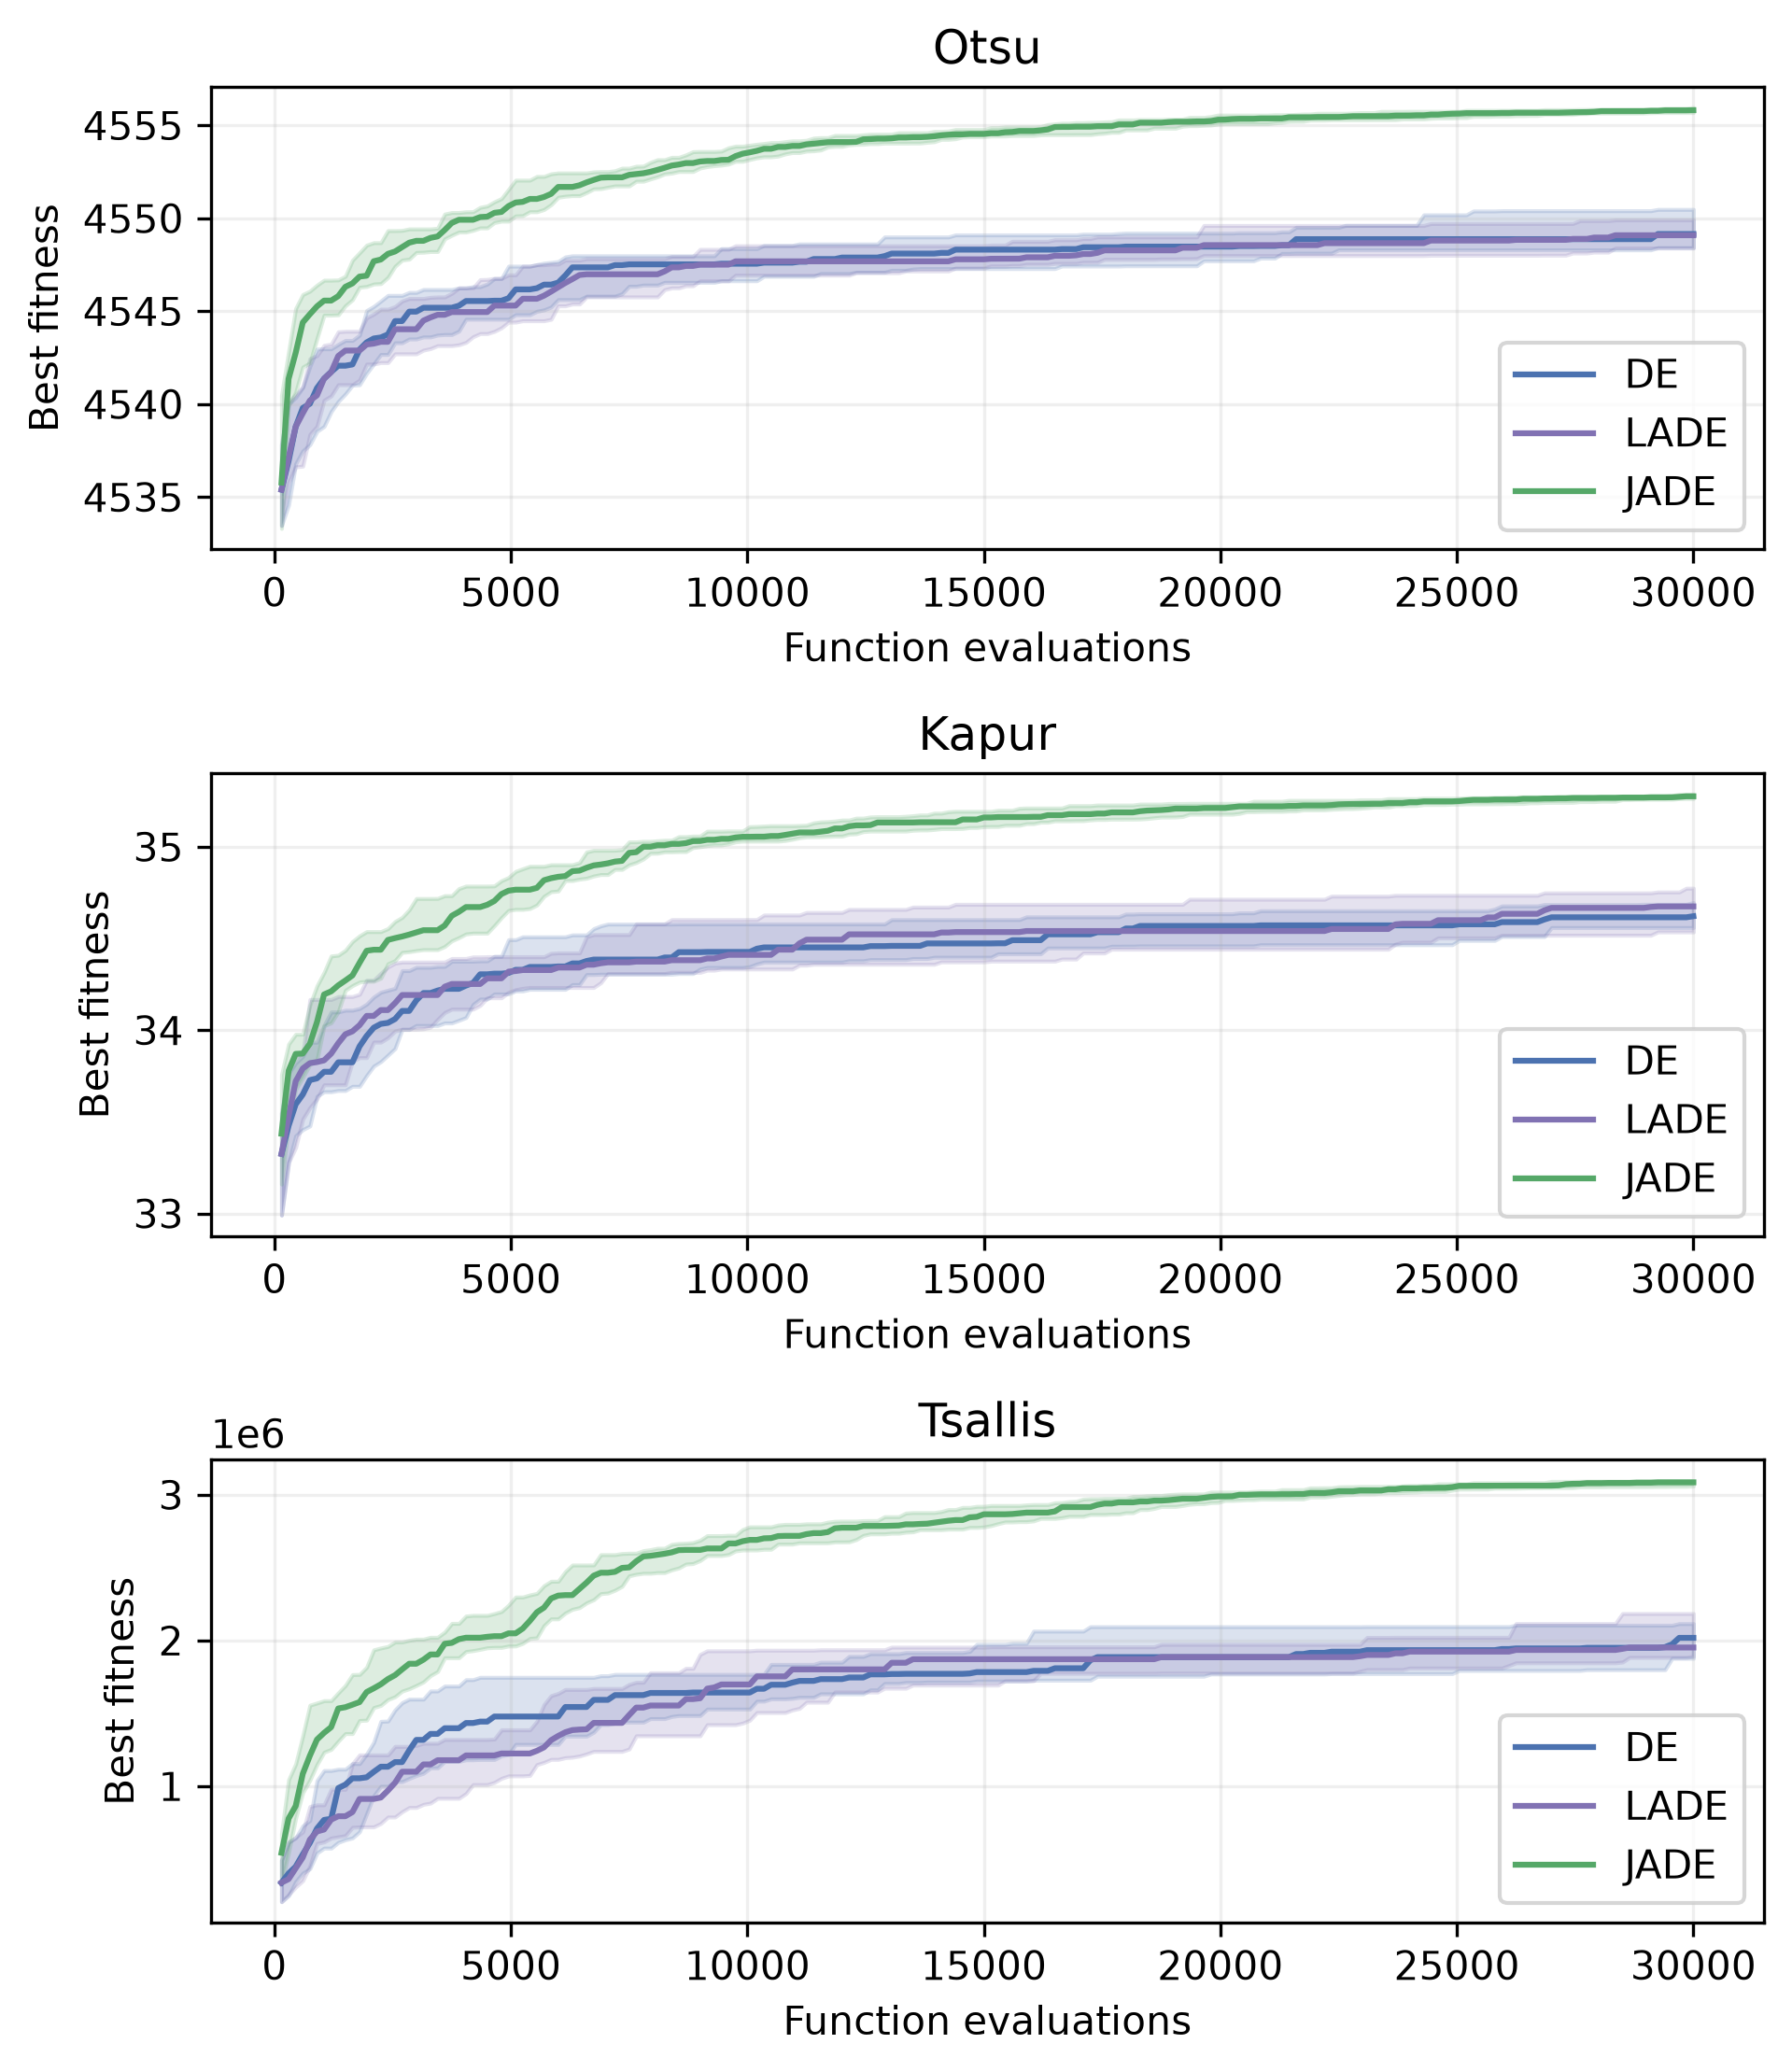
\includegraphics[width=\textwidth]{exp1_convergence.png}

\caption{Best-so-far fitness for img1 at $K=12$. Lines show the median over 30 runs and shaded bands show the interquartile range. Each panel uses its own objective scale; fitness values are not comparable across objectives.}

\label{fig:bsd_convergence}

\end{figure}

Figure~\ref{fig:bsd_convergence} compares convergence under an equal evaluation budget. Best-so-far fitness is retained independently of the current population in LADE, so its curves remain nondecreasing despite acceptance of some worse trials. These curves describe one illustrative image and do not alone establish a dataset-wide convergence advantage.

\subsection{Visual Segmentation Results}

\begin{figure}[htbp]

\centering

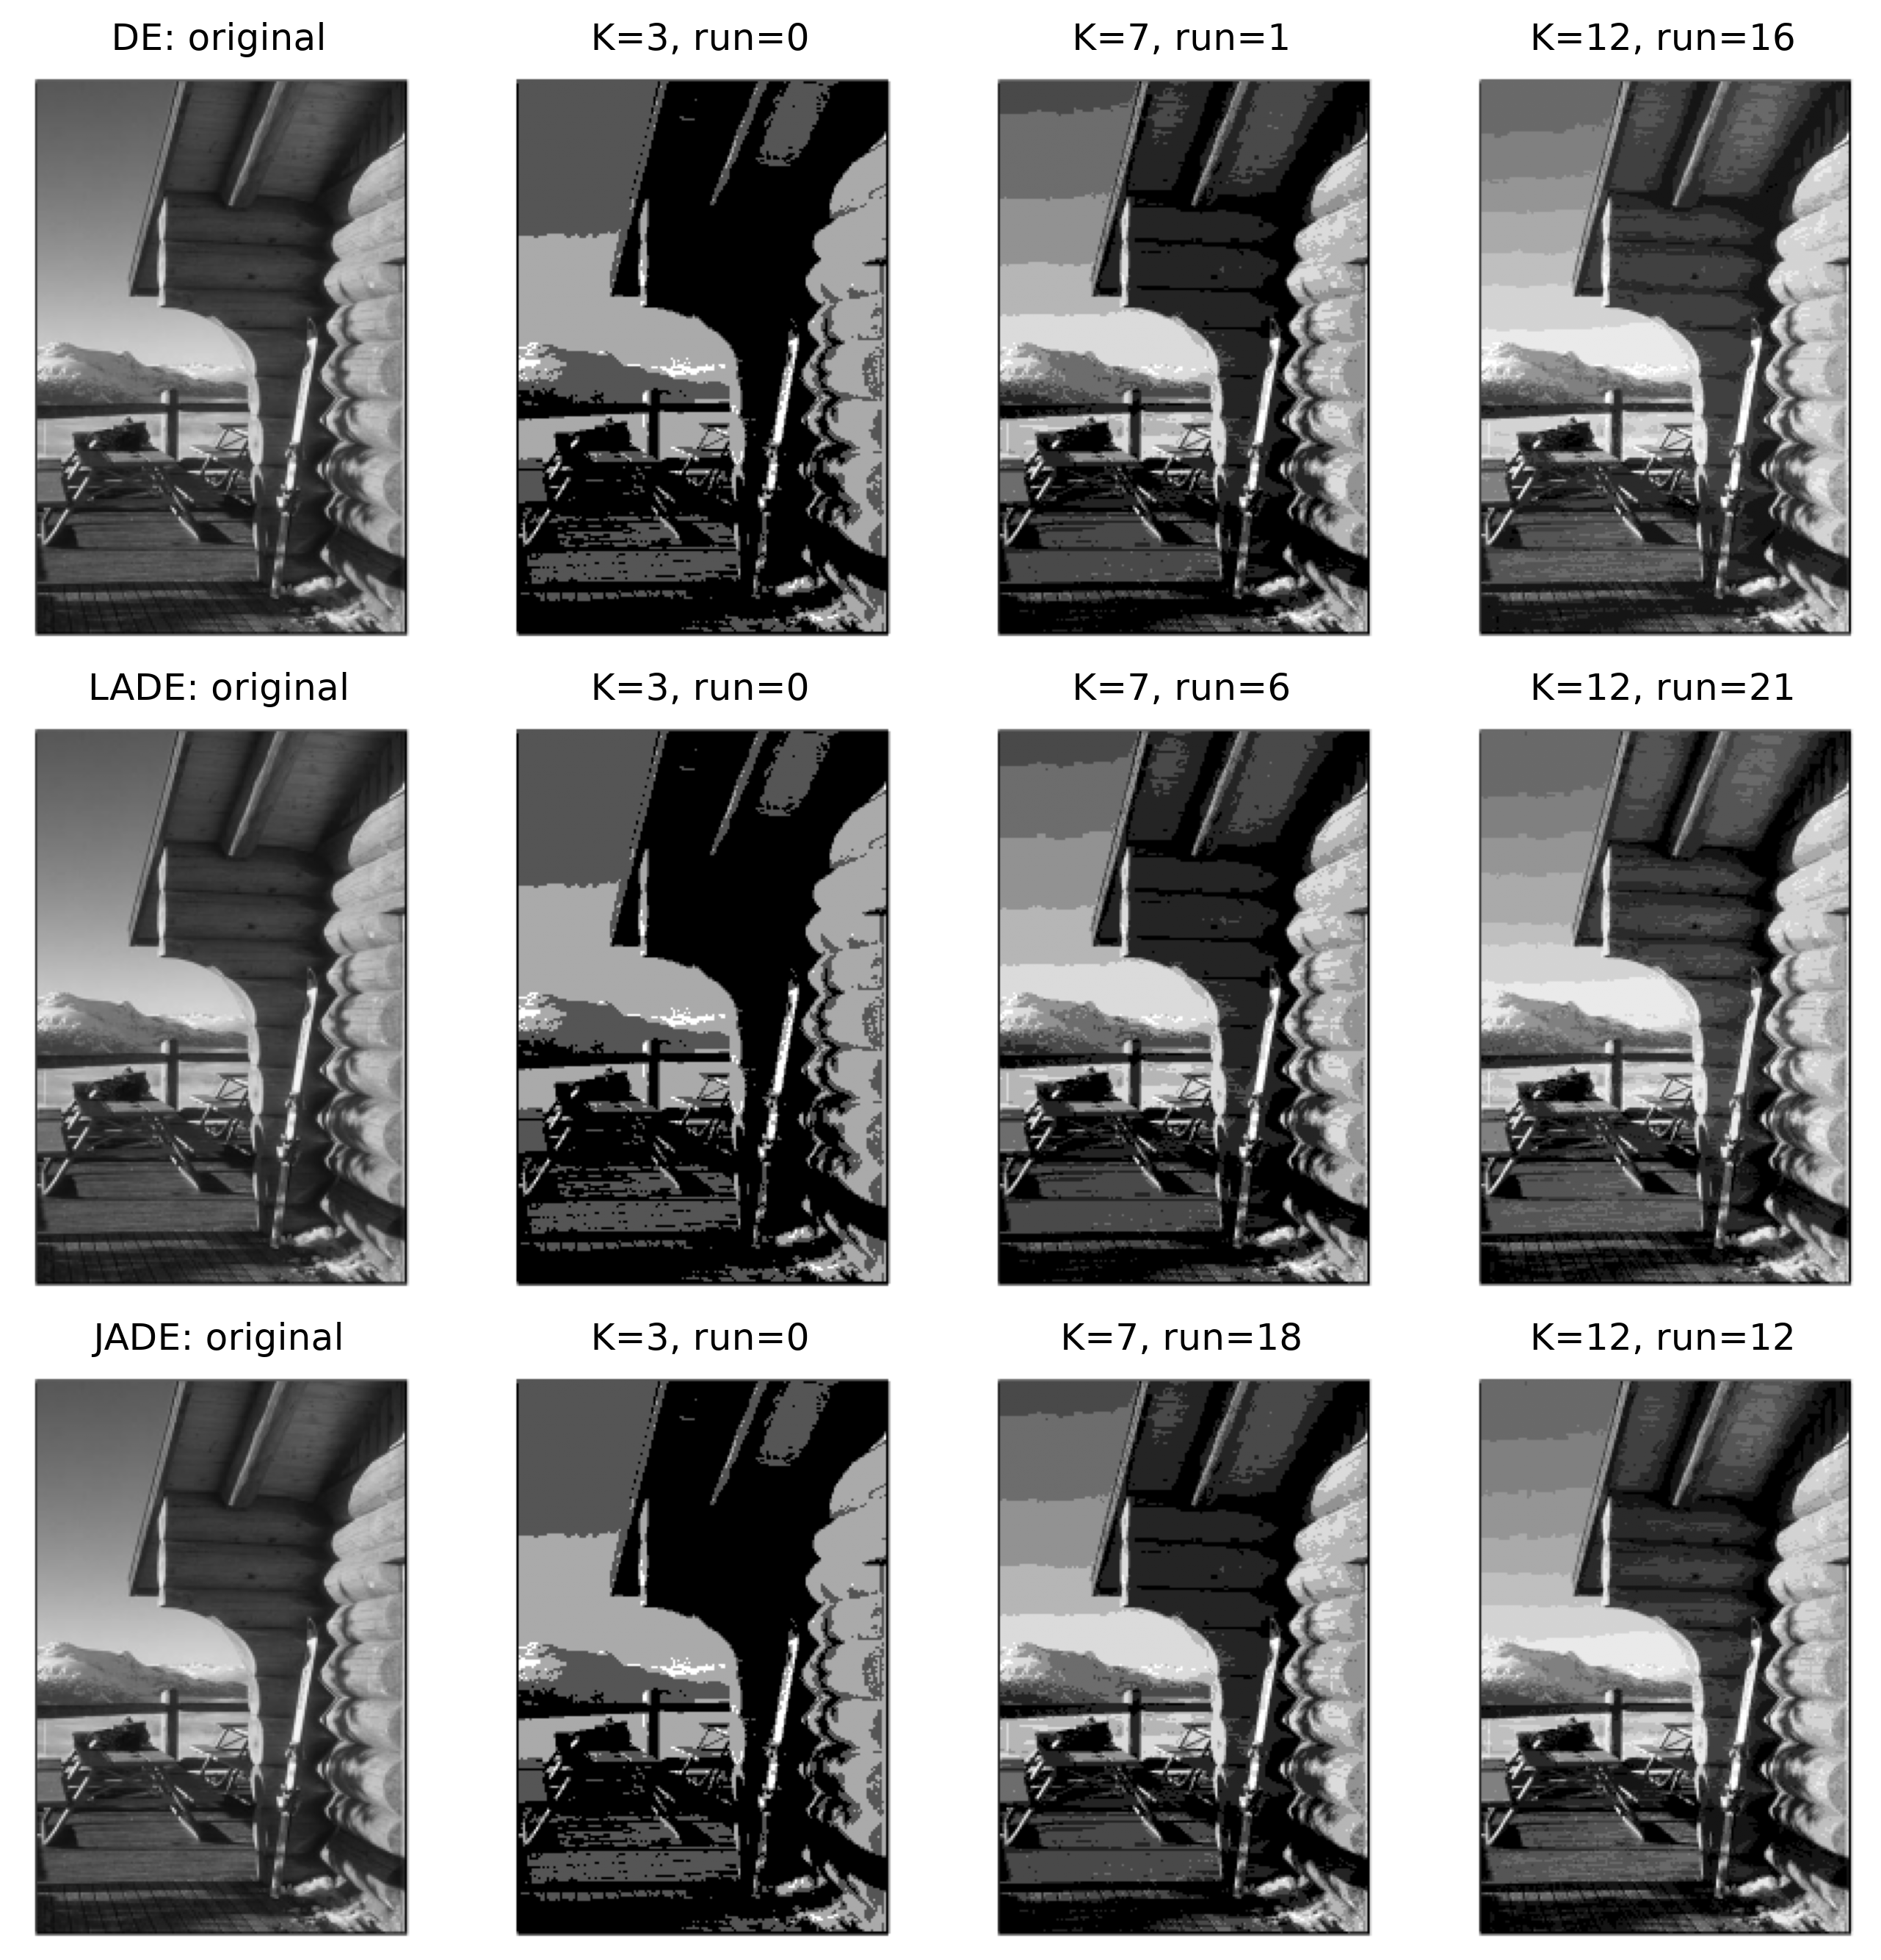
\includegraphics[width=0.9\textwidth]{exp1_segmentation_otsu.png}

\caption{Original and segmented img1 under Otsu at $K=3,7,12$. DE occupies the first row, LADE the second, and JADE the third. Each solution is selected by fitness closest to the median of its 30 runs (ties use the lowest run index). Class intensities are spread evenly for display; PSNR and SSIM are computed using class means instead.}

\label{fig:bsd-segmentation-otsu}

\end{figure}

\begin{figure}[htbp]

\centering

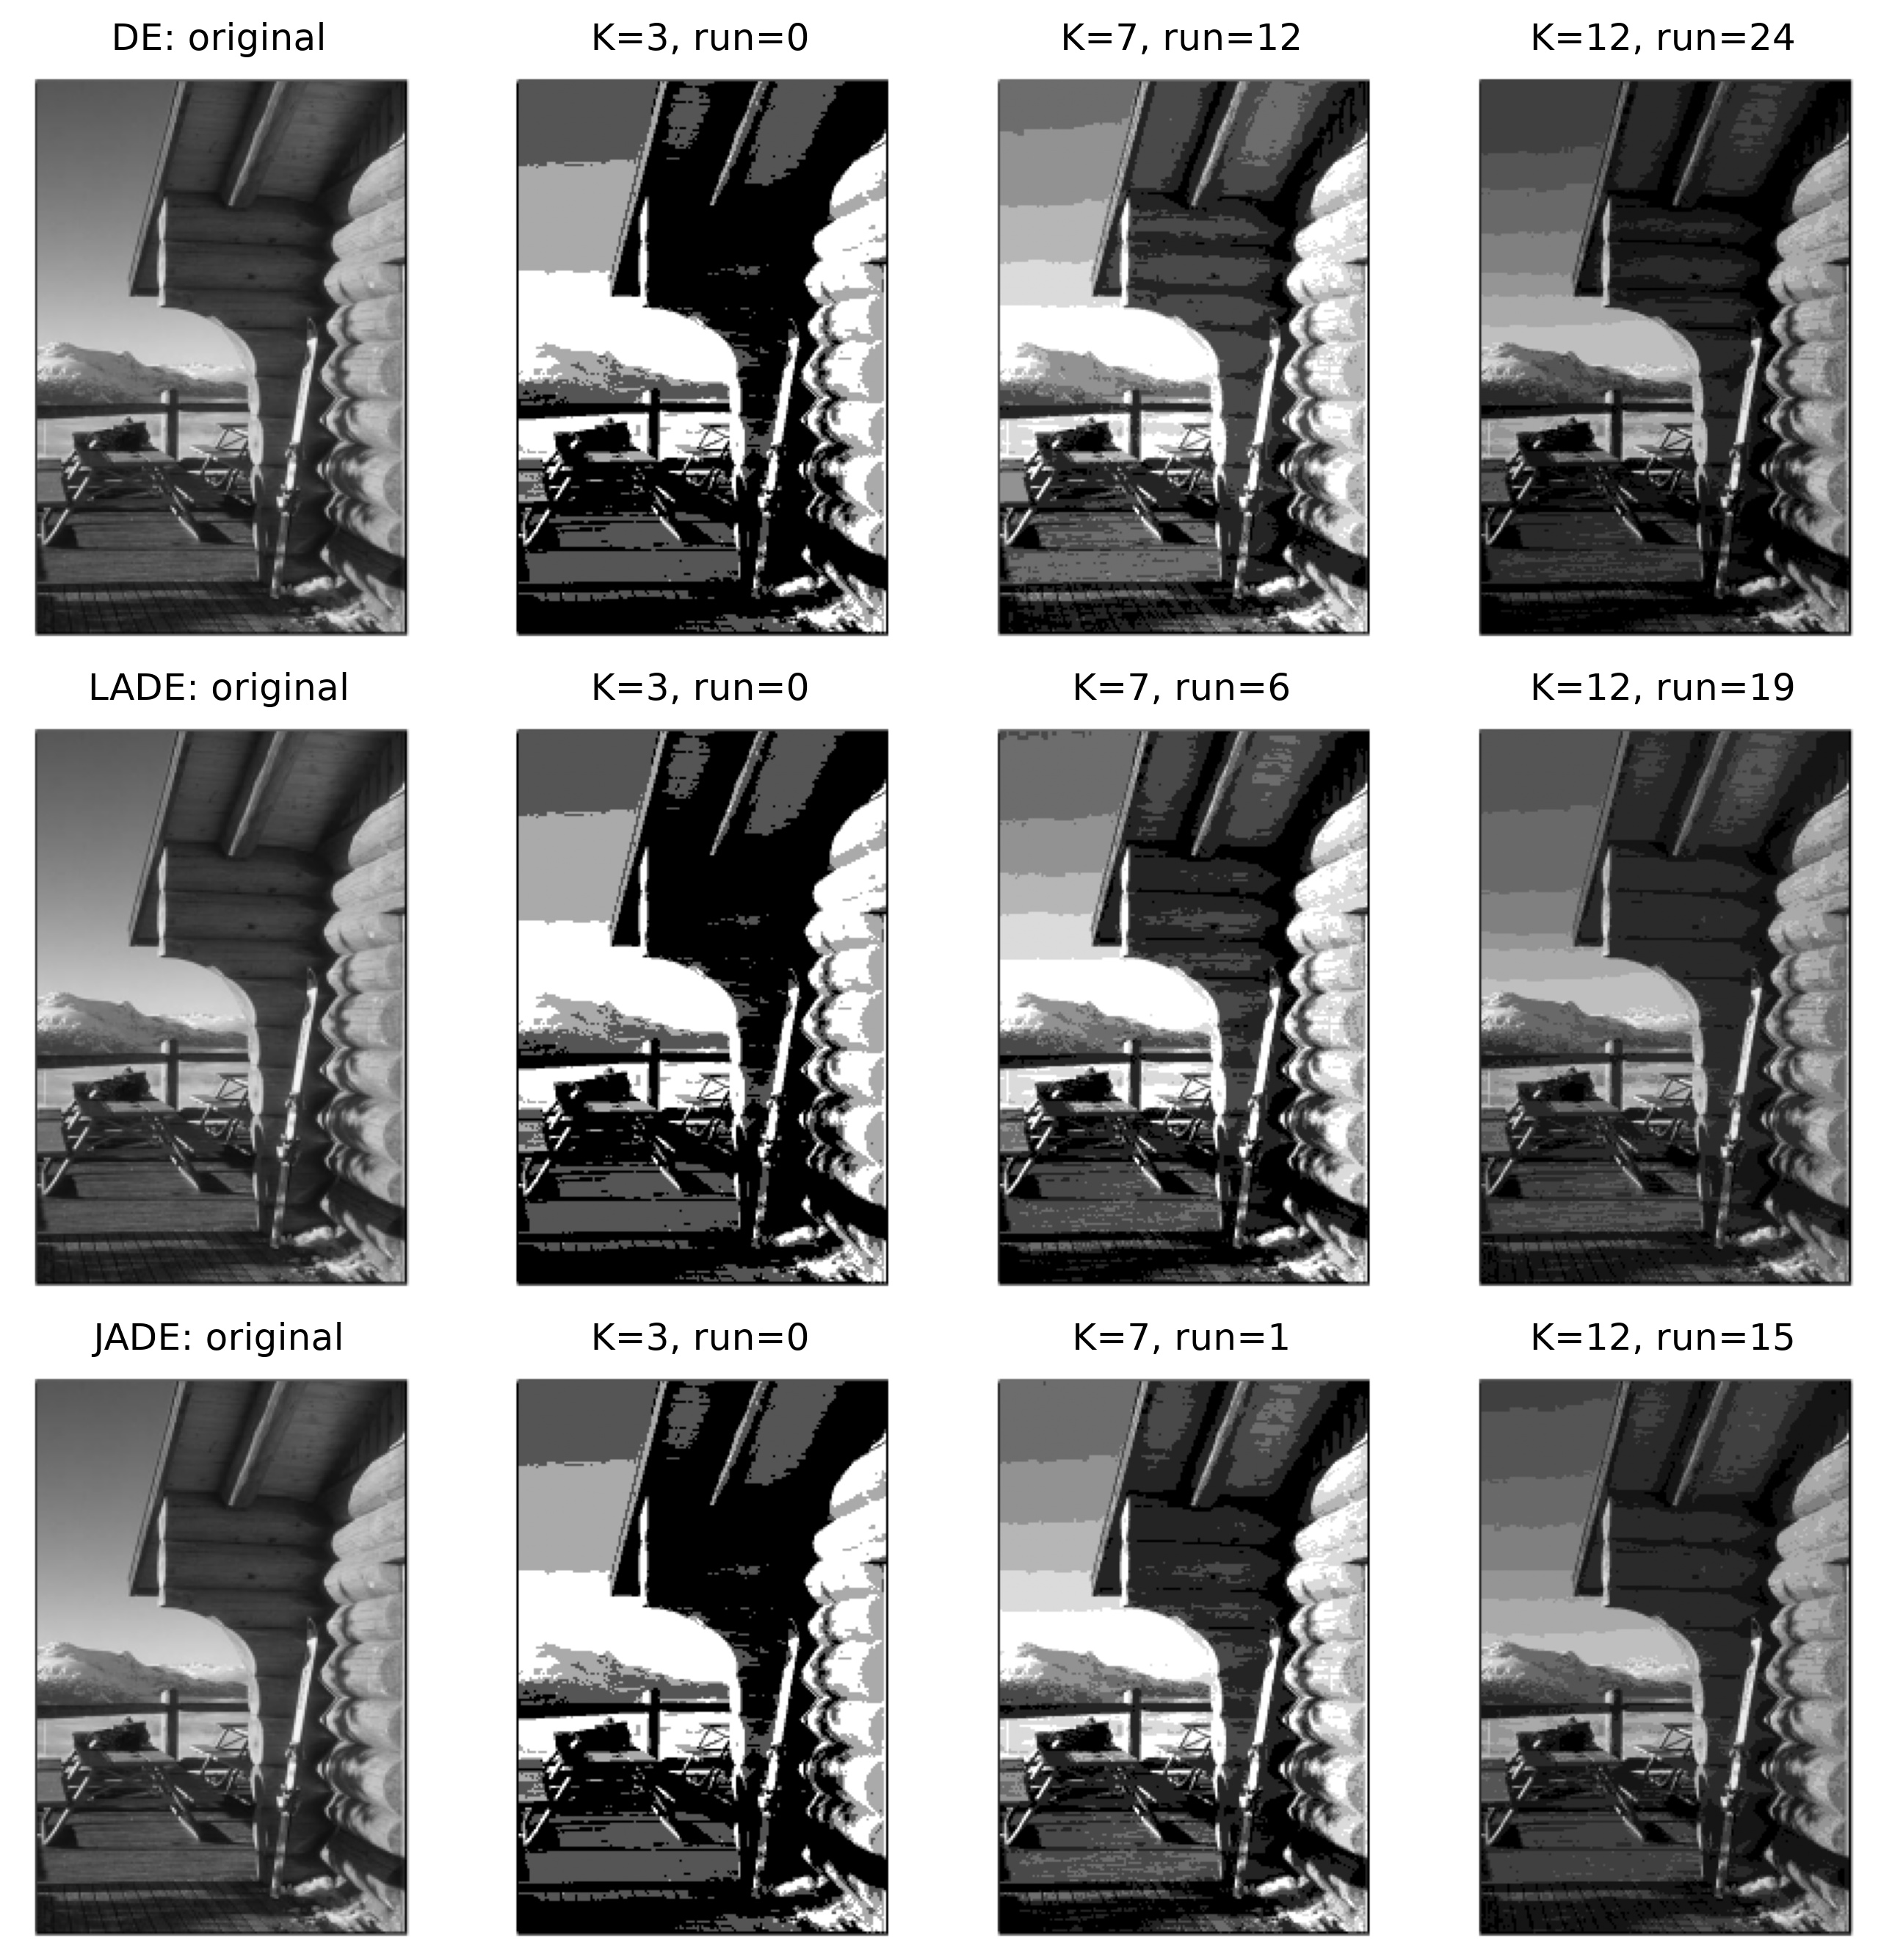
\includegraphics[width=0.9\textwidth]{exp1_segmentation_kapur.png}

\caption{Original and segmented img1 under Kapur at $K=3,7,12$. DE occupies the first row, LADE the second, and JADE the third. Each solution is selected by fitness closest to the median of its 30 runs (ties use the lowest run index). Class intensities are spread evenly for display; PSNR and SSIM are computed using class means instead.}

\label{fig:bsd-segmentation-kapur}

\end{figure}

\begin{figure}[htbp]

\centering

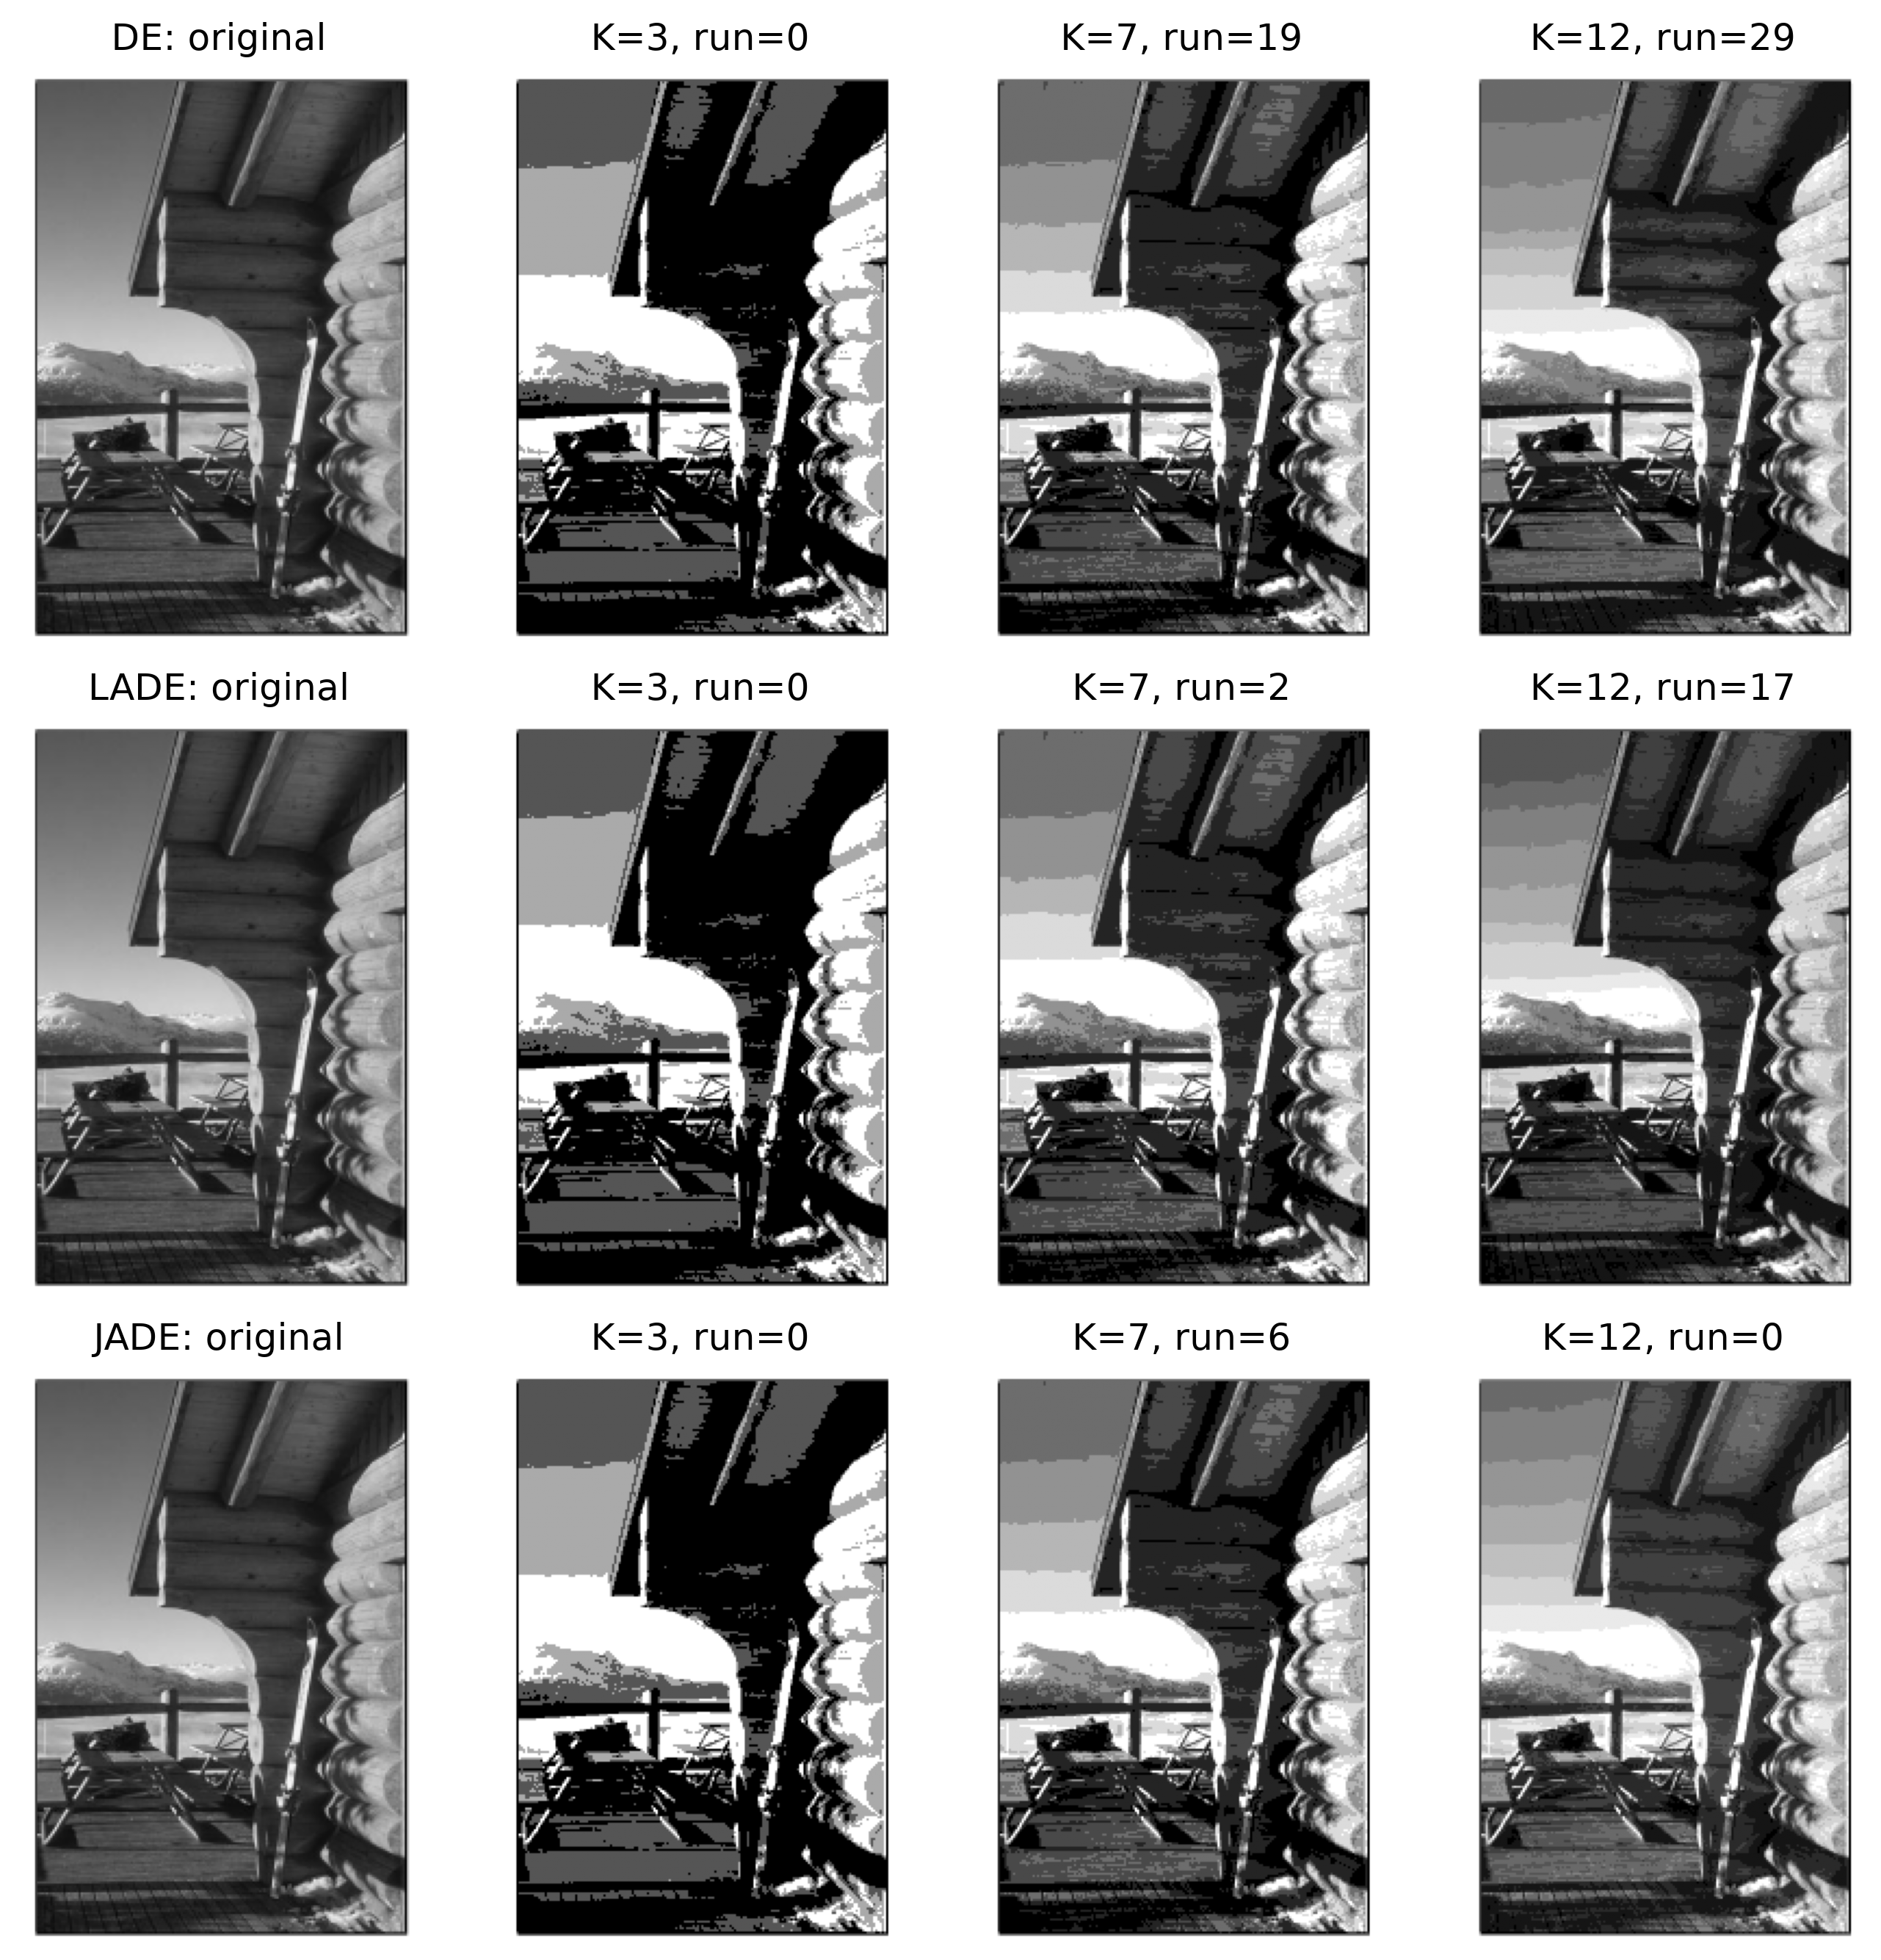
\includegraphics[width=0.9\textwidth]{exp1_segmentation_tsallis.png}

\caption{Original and segmented img1 under Tsallis at $K=3,7,12$. DE occupies the first row, LADE the second, and JADE the third. Each solution is selected by fitness closest to the median of its 30 runs (ties use the lowest run index). Class intensities are spread evenly for display; PSNR and SSIM are computed using class means instead.}

\label{fig:bsd-segmentation-tsallis}

\end{figure}

\clearpage

\subsection{Execution Time}

\begin{figure}[htbp]

\centering

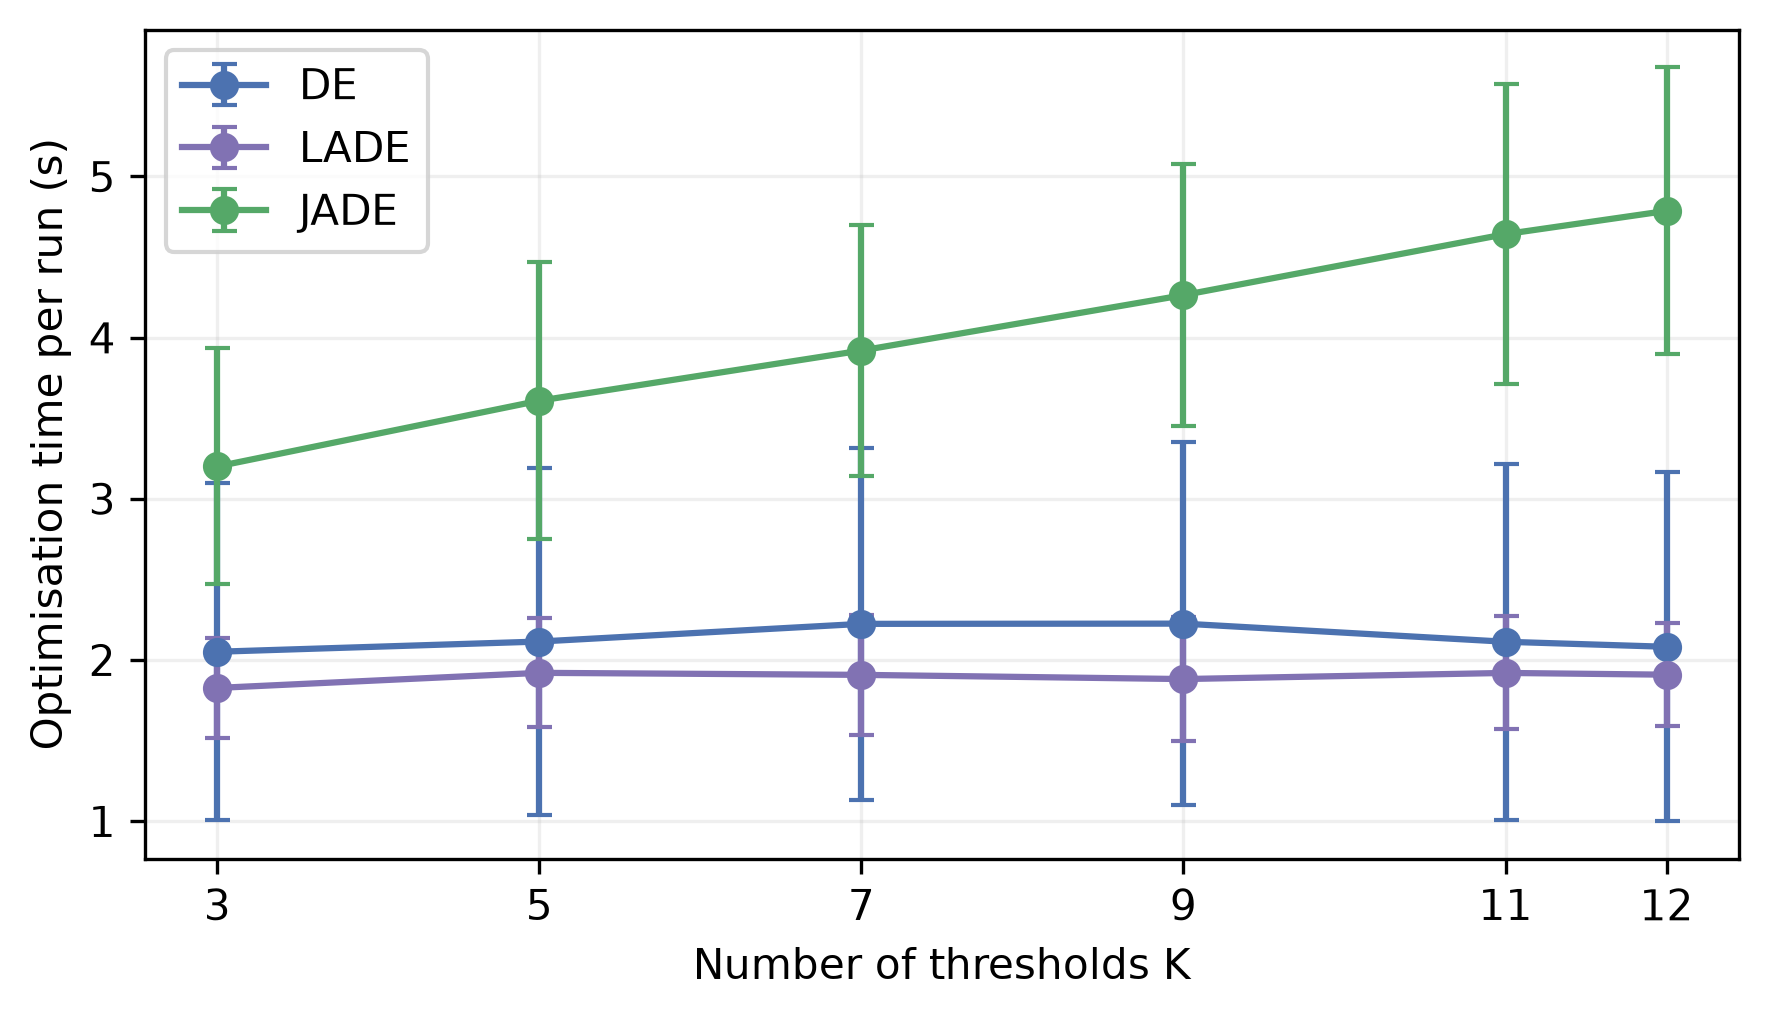
\includegraphics[width=0.8\textwidth]{exp1_runtime.png}

\caption{Mean recorded optimisation time versus $K$ for DE, LADE and JADE. Error bars show sample standard deviation over 900 runs per algorithm and threshold count (10 images, three objectives, 30 runs). DE, LADE and JADE were run in separate sweeps, so machine load and worker settings can influence this comparison.}

\label{fig:bsd-runtime}

\end{figure}

Timing covers optimiser execution and objective evaluations using \texttt{time.perf\_counter}; image loading, histogram preparation, exact reference computation, metric calculation and result writing are excluded. The saved results do not record hardware or worker counts, so runtime differences cannot be attributed exclusively to algorithm design.

\subsection{Discussion of Experiment 1}

JADE does not lead every reconstruction metric. At $K=12$, it has the highest reported mean PSNR and SSIM under Otsu and Kapur. Under Tsallis, however, its mean PSNR (28.5486 dB) is lower than DE (28.5999 dB) and LADE (28.6270 dB), while its mean SSIM (0.9138) is higher. These descriptive results show that the comparison depends on both the objective function and the evaluation metric. The pooled standard deviations remain descriptive summaries that combine differences between images with stochastic variation within images; therefore, they do not establish JADE stability or faster convergence without per-image run summaries and convergence evidence. Overall, the experiment supports the expected improvement in reconstruction with more thresholds and shows that objective choice affects the relative ranking of algorithms more strongly than any single optimiser dominates across all metrics.

\section{Experiment 2: CHAOS MRI Images}

\label{sec:experiment2}

\subsection{Experimental Objective}

Results for JADE on 15 CHAOS MRI images, using Otsu, Kapur and Tsallis ($q=0.8$), with $K\in\{3,5,7,9,11,12\}$. Each image--objective--threshold combination contains 30 runs with 30,000 function evaluations per run.

\subsection{Ground-Truth Mask Matching}

--

\subsection{Reconstruction Metrics}

Tables report pooled means and sample standard deviations across images and runs. Dashes indicate unavailable results.

\begin{table}[htbp]
\centering
\small
\caption{PSNR (dB) on CHAOS MRI using Otsu: pooled mean $\pm$ sample standard deviation across 450 observations per entry (15 slices, 30 runs each). Dashes indicate unavailable results.}
\label{tab:chaos-otsu-psnr}
\resizebox{\textwidth}{!}{%
\begin{tabular}{lcccccc}
\toprule
Algorithm & $K=3$ & $K=5$ & $K=7$ & $K=9$ & $K=11$ & $K=12$ \\
\midrule
DE & -- & -- & -- & -- & -- & -- \\
JADE & $27.8831 \pm 0.8927$ & $31.4137 \pm 0.8965$ & $33.9062 \pm 0.9500$ & $35.8692 \pm 0.9422$ & $37.4321 \pm 0.9455$ & $38.1275 \pm 0.9562$ \\
SHADE & -- & -- & -- & -- & -- & -- \\
L-SHADE & -- & -- & -- & -- & -- & -- \\
LADE & -- & -- & -- & -- & -- & -- \\
\bottomrule
\end{tabular}%
}
\end{table}

\begin{table}[htbp]
\centering
\small
\caption{SSIM on CHAOS MRI using Otsu: pooled mean $\pm$ sample standard deviation across 450 observations per entry (15 slices, 30 runs each). Dashes indicate unavailable results.}
\label{tab:chaos-otsu-ssim}
\resizebox{\textwidth}{!}{%
\begin{tabular}{lcccccc}
\toprule
Algorithm & $K=3$ & $K=5$ & $K=7$ & $K=9$ & $K=11$ & $K=12$ \\
\midrule
DE & -- & -- & -- & -- & -- & -- \\
JADE & $0.8664 \pm 0.0411$ & $0.9241 \pm 0.0219$ & $0.9499 \pm 0.0144$ & $0.9643 \pm 0.0110$ & $0.9730 \pm 0.0085$ & $0.9763 \pm 0.0077$ \\
SHADE & -- & -- & -- & -- & -- & -- \\
L-SHADE & -- & -- & -- & -- & -- & -- \\
LADE & -- & -- & -- & -- & -- & -- \\
\bottomrule
\end{tabular}%
}
\end{table}

\begin{table}[htbp]
\centering
\small
\caption{Uniformity on CHAOS MRI using Otsu: pooled mean $\pm$ sample standard deviation across 450 observations per entry (15 slices, 30 runs each). Dashes indicate unavailable results.}
\label{tab:chaos-otsu-uniformity}
\resizebox{\textwidth}{!}{%
\begin{tabular}{lcccccc}
\toprule
Algorithm & $K=3$ & $K=5$ & $K=7$ & $K=9$ & $K=11$ & $K=12$ \\
\midrule
DE & -- & -- & -- & -- & -- & -- \\
JADE & $0.9900 \pm 0.0020$ & $0.9926 \pm 0.0015$ & $0.9942 \pm 0.0012$ & $0.9952 \pm 0.0010$ & $0.9959 \pm 0.0008$ & $0.9962 \pm 0.0008$ \\
SHADE & -- & -- & -- & -- & -- & -- \\
L-SHADE & -- & -- & -- & -- & -- & -- \\
LADE & -- & -- & -- & -- & -- & -- \\
\bottomrule
\end{tabular}%
}
\end{table}

\begin{table}[htbp]
\centering
\small
\caption{Class separability on CHAOS MRI using Otsu: pooled mean $\pm$ sample standard deviation across 450 observations per entry (15 slices, 30 runs each). Dashes indicate unavailable results.}
\label{tab:chaos-otsu-class_separability}
\resizebox{\textwidth}{!}{%
\begin{tabular}{lcccccc}
\toprule
Algorithm & $K=3$ & $K=5$ & $K=7$ & $K=9$ & $K=11$ & $K=12$ \\
\midrule
DE & -- & -- & -- & -- & -- & -- \\
JADE & $0.9760 \pm 0.0076$ & $0.9894 \pm 0.0030$ & $0.9941 \pm 0.0015$ & $0.9962 \pm 0.0010$ & $0.9974 \pm 0.0006$ & $0.9978 \pm 0.0006$ \\
SHADE & -- & -- & -- & -- & -- & -- \\
L-SHADE & -- & -- & -- & -- & -- & -- \\
LADE & -- & -- & -- & -- & -- & -- \\
\bottomrule
\end{tabular}%
}
\end{table}

\begin{table}[htbp]
\centering
\small
\caption{PSNR (dB) on CHAOS MRI using Kapur: pooled mean $\pm$ sample standard deviation across 450 observations per entry (15 slices, 30 runs each). Dashes indicate unavailable results.}
\label{tab:chaos-kapur-psnr}
\resizebox{\textwidth}{!}{%
\begin{tabular}{lcccccc}
\toprule
Algorithm & $K=3$ & $K=5$ & $K=7$ & $K=9$ & $K=11$ & $K=12$ \\
\midrule
DE & -- & -- & -- & -- & -- & -- \\
JADE & $23.9215 \pm 3.2645$ & $29.5511 \pm 1.0776$ & $32.5735 \pm 0.8779$ & $34.6452 \pm 0.9256$ & $36.3602 \pm 0.7879$ & $37.0384 \pm 0.7995$ \\
SHADE & -- & -- & -- & -- & -- & -- \\
L-SHADE & -- & -- & -- & -- & -- & -- \\
LADE & -- & -- & -- & -- & -- & -- \\
\bottomrule
\end{tabular}%
}
\end{table}

\begin{table}[htbp]
\centering
\small
\caption{SSIM on CHAOS MRI using Kapur: pooled mean $\pm$ sample standard deviation across 450 observations per entry (15 slices, 30 runs each). Dashes indicate unavailable results.}
\label{tab:chaos-kapur-ssim}
\resizebox{\textwidth}{!}{%
\begin{tabular}{lcccccc}
\toprule
Algorithm & $K=3$ & $K=5$ & $K=7$ & $K=9$ & $K=11$ & $K=12$ \\
\midrule
DE & -- & -- & -- & -- & -- & -- \\
JADE & $0.6508 \pm 0.2917$ & $0.9106 \pm 0.0268$ & $0.9396 \pm 0.0163$ & $0.9550 \pm 0.0134$ & $0.9660 \pm 0.0104$ & $0.9695 \pm 0.0097$ \\
SHADE & -- & -- & -- & -- & -- & -- \\
L-SHADE & -- & -- & -- & -- & -- & -- \\
LADE & -- & -- & -- & -- & -- & -- \\
\bottomrule
\end{tabular}%
}
\end{table}

\begin{table}[htbp]
\centering
\small
\caption{Uniformity on CHAOS MRI using Kapur: pooled mean $\pm$ sample standard deviation across 450 observations per entry (15 slices, 30 runs each). Dashes indicate unavailable results.}
\label{tab:chaos-kapur-uniformity}
\resizebox{\textwidth}{!}{%
\begin{tabular}{lcccccc}
\toprule
Algorithm & $K=3$ & $K=5$ & $K=7$ & $K=9$ & $K=11$ & $K=12$ \\
\midrule
DE & -- & -- & -- & -- & -- & -- \\
JADE & $0.9654 \pm 0.0376$ & $0.9885 \pm 0.0031$ & $0.9921 \pm 0.0015$ & $0.9937 \pm 0.0013$ & $0.9948 \pm 0.0009$ & $0.9952 \pm 0.0009$ \\
SHADE & -- & -- & -- & -- & -- & -- \\
L-SHADE & -- & -- & -- & -- & -- & -- \\
LADE & -- & -- & -- & -- & -- & -- \\
\bottomrule
\end{tabular}%
}
\end{table}

\begin{table}[htbp]
\centering
\small
\caption{Class separability on CHAOS MRI using Kapur: pooled mean $\pm$ sample standard deviation across 450 observations per entry (15 slices, 30 runs each). Dashes indicate unavailable results.}
\label{tab:chaos-kapur-class_separability}
\resizebox{\textwidth}{!}{%
\begin{tabular}{lcccccc}
\toprule
Algorithm & $K=3$ & $K=5$ & $K=7$ & $K=9$ & $K=11$ & $K=12$ \\
\midrule
DE & -- & -- & -- & -- & -- & -- \\
JADE & $0.9105 \pm 0.0956$ & $0.9835 \pm 0.0056$ & $0.9919 \pm 0.0023$ & $0.9950 \pm 0.0015$ & $0.9966 \pm 0.0010$ & $0.9971 \pm 0.0009$ \\
SHADE & -- & -- & -- & -- & -- & -- \\
L-SHADE & -- & -- & -- & -- & -- & -- \\
LADE & -- & -- & -- & -- & -- & -- \\
\bottomrule
\end{tabular}%
}
\end{table}

\begin{table}[htbp]
\centering
\small
\caption{PSNR (dB) on CHAOS MRI using Tsallis ($q=0.8$): pooled mean $\pm$ sample standard deviation across 450 observations per entry (15 slices, 30 runs each). Dashes indicate unavailable results.}
\label{tab:chaos-tsallis-psnr}
\resizebox{\textwidth}{!}{%
\begin{tabular}{lcccccc}
\toprule
Algorithm & $K=3$ & $K=5$ & $K=7$ & $K=9$ & $K=11$ & $K=12$ \\
\midrule
DE & -- & -- & -- & -- & -- & -- \\
JADE & $19.2181 \pm 1.6513$ & $21.6337 \pm 1.1302$ & $23.2396 \pm 1.2537$ & $24.9296 \pm 1.4644$ & $28.0504 \pm 2.9103$ & $31.8409 \pm 3.9607$ \\
SHADE & -- & -- & -- & -- & -- & -- \\
L-SHADE & -- & -- & -- & -- & -- & -- \\
LADE & -- & -- & -- & -- & -- & -- \\
\bottomrule
\end{tabular}%
}
\end{table}

\begin{table}[htbp]
\centering
\small
\caption{SSIM on CHAOS MRI using Tsallis ($q=0.8$): pooled mean $\pm$ sample standard deviation across 450 observations per entry (15 slices, 30 runs each). Dashes indicate unavailable results.}
\label{tab:chaos-tsallis-ssim}
\resizebox{\textwidth}{!}{%
\begin{tabular}{lcccccc}
\toprule
Algorithm & $K=3$ & $K=5$ & $K=7$ & $K=9$ & $K=11$ & $K=12$ \\
\midrule
DE & -- & -- & -- & -- & -- & -- \\
JADE & $0.2650 \pm 0.0370$ & $0.3347 \pm 0.0436$ & $0.3878 \pm 0.0616$ & $0.4550 \pm 0.0676$ & $0.6016 \pm 0.1498$ & $0.7632 \pm 0.1805$ \\
SHADE & -- & -- & -- & -- & -- & -- \\
L-SHADE & -- & -- & -- & -- & -- & -- \\
LADE & -- & -- & -- & -- & -- & -- \\
\bottomrule
\end{tabular}%
}
\end{table}

\begin{table}[htbp]
\centering
\small
\caption{Uniformity on CHAOS MRI using Tsallis ($q=0.8$): pooled mean $\pm$ sample standard deviation across 450 observations per entry (15 slices, 30 runs each). Dashes indicate unavailable results.}
\label{tab:chaos-tsallis-uniformity}
\resizebox{\textwidth}{!}{%
\begin{tabular}{lcccccc}
\toprule
Algorithm & $K=3$ & $K=5$ & $K=7$ & $K=9$ & $K=11$ & $K=12$ \\
\midrule
DE & -- & -- & -- & -- & -- & -- \\
JADE & $0.9224 \pm 0.0329$ & $0.9290 \pm 0.0186$ & $0.9308 \pm 0.0199$ & $0.9388 \pm 0.0211$ & $0.9588 \pm 0.0216$ & $0.9771 \pm 0.0180$ \\
SHADE & -- & -- & -- & -- & -- & -- \\
L-SHADE & -- & -- & -- & -- & -- & -- \\
LADE & -- & -- & -- & -- & -- & -- \\
\bottomrule
\end{tabular}%
}
\end{table}

\begin{table}[htbp]
\centering
\small
\caption{Class separability on CHAOS MRI using Tsallis ($q=0.8$): pooled mean $\pm$ sample standard deviation across 450 observations per entry (15 slices, 30 runs each). Dashes indicate unavailable results.}
\label{tab:chaos-tsallis-class_separability}
\resizebox{\textwidth}{!}{%
\begin{tabular}{lcccccc}
\toprule
Algorithm & $K=3$ & $K=5$ & $K=7$ & $K=9$ & $K=11$ & $K=12$ \\
\midrule
DE & -- & -- & -- & -- & -- & -- \\
JADE & $0.8128 \pm 0.0919$ & $0.8981 \pm 0.0340$ & $0.9262 \pm 0.0348$ & $0.9507 \pm 0.0195$ & $0.9717 \pm 0.0165$ & $0.9844 \pm 0.0144$ \\
SHADE & -- & -- & -- & -- & -- & -- \\
L-SHADE & -- & -- & -- & -- & -- & -- \\
LADE & -- & -- & -- & -- & -- & -- \\
\bottomrule
\end{tabular}%
}
\end{table}

\subsection{Ground-Truth Segmentation Performance}

\begin{table}[htbp]
\centering
\small
\caption{Dice coefficient on CHAOS MRI using Otsu: pooled mean $\pm$ sample standard deviation across 450 observations per entry (15 slices, 30 runs each). Dashes indicate unavailable results.}
\label{tab:chaos-otsu-dice}
\resizebox{\textwidth}{!}{%
\begin{tabular}{lcccccc}
\toprule
Algorithm & $K=3$ & $K=5$ & $K=7$ & $K=9$ & $K=11$ & $K=12$ \\
\midrule
DE & -- & -- & -- & -- & -- & -- \\
JADE & -- & -- & -- & -- & -- & -- \\
SHADE & -- & -- & -- & -- & -- & -- \\
L-SHADE & -- & -- & -- & -- & -- & -- \\
LADE & -- & -- & -- & -- & -- & -- \\
\bottomrule
\end{tabular}%
}
\end{table}

\begin{table}[htbp]
\centering
\small
\caption{Jaccard index on CHAOS MRI using Otsu: pooled mean $\pm$ sample standard deviation across 450 observations per entry (15 slices, 30 runs each). Dashes indicate unavailable results.}
\label{tab:chaos-otsu-jaccard}
\resizebox{\textwidth}{!}{%
\begin{tabular}{lcccccc}
\toprule
Algorithm & $K=3$ & $K=5$ & $K=7$ & $K=9$ & $K=11$ & $K=12$ \\
\midrule
DE & -- & -- & -- & -- & -- & -- \\
JADE & -- & -- & -- & -- & -- & -- \\
SHADE & -- & -- & -- & -- & -- & -- \\
L-SHADE & -- & -- & -- & -- & -- & -- \\
LADE & -- & -- & -- & -- & -- & -- \\
\bottomrule
\end{tabular}%
}
\end{table}

\begin{table}[htbp]
\centering
\small
\caption{Dice coefficient on CHAOS MRI using Kapur: pooled mean $\pm$ sample standard deviation across 450 observations per entry (15 slices, 30 runs each). Dashes indicate unavailable results.}
\label{tab:chaos-kapur-dice}
\resizebox{\textwidth}{!}{%
\begin{tabular}{lcccccc}
\toprule
Algorithm & $K=3$ & $K=5$ & $K=7$ & $K=9$ & $K=11$ & $K=12$ \\
\midrule
DE & -- & -- & -- & -- & -- & -- \\
JADE & -- & -- & -- & -- & -- & -- \\
SHADE & -- & -- & -- & -- & -- & -- \\
L-SHADE & -- & -- & -- & -- & -- & -- \\
LADE & -- & -- & -- & -- & -- & -- \\
\bottomrule
\end{tabular}%
}
\end{table}

\begin{table}[htbp]
\centering
\small
\caption{Jaccard index on CHAOS MRI using Kapur: pooled mean $\pm$ sample standard deviation across 450 observations per entry (15 slices, 30 runs each). Dashes indicate unavailable results.}
\label{tab:chaos-kapur-jaccard}
\resizebox{\textwidth}{!}{%
\begin{tabular}{lcccccc}
\toprule
Algorithm & $K=3$ & $K=5$ & $K=7$ & $K=9$ & $K=11$ & $K=12$ \\
\midrule
DE & -- & -- & -- & -- & -- & -- \\
JADE & -- & -- & -- & -- & -- & -- \\
SHADE & -- & -- & -- & -- & -- & -- \\
L-SHADE & -- & -- & -- & -- & -- & -- \\
LADE & -- & -- & -- & -- & -- & -- \\
\bottomrule
\end{tabular}%
}
\end{table}

\begin{table}[htbp]
\centering
\small
\caption{Dice coefficient on CHAOS MRI using Tsallis ($q=0.8$): pooled mean $\pm$ sample standard deviation across 450 observations per entry (15 slices, 30 runs each). Dashes indicate unavailable results.}
\label{tab:chaos-tsallis-dice}
\resizebox{\textwidth}{!}{%
\begin{tabular}{lcccccc}
\toprule
Algorithm & $K=3$ & $K=5$ & $K=7$ & $K=9$ & $K=11$ & $K=12$ \\
\midrule
DE & -- & -- & -- & -- & -- & -- \\
JADE & -- & -- & -- & -- & -- & -- \\
SHADE & -- & -- & -- & -- & -- & -- \\
L-SHADE & -- & -- & -- & -- & -- & -- \\
LADE & -- & -- & -- & -- & -- & -- \\
\bottomrule
\end{tabular}%
}
\end{table}

\begin{table}[htbp]
\centering
\small
\caption{Jaccard index on CHAOS MRI using Tsallis ($q=0.8$): pooled mean $\pm$ sample standard deviation across 450 observations per entry (15 slices, 30 runs each). Dashes indicate unavailable results.}
\label{tab:chaos-tsallis-jaccard}
\resizebox{\textwidth}{!}{%
\begin{tabular}{lcccccc}
\toprule
Algorithm & $K=3$ & $K=5$ & $K=7$ & $K=9$ & $K=11$ & $K=12$ \\
\midrule
DE & -- & -- & -- & -- & -- & -- \\
JADE & -- & -- & -- & -- & -- & -- \\
SHADE & -- & -- & -- & -- & -- & -- \\
L-SHADE & -- & -- & -- & -- & -- & -- \\
LADE & -- & -- & -- & -- & -- & -- \\
\bottomrule
\end{tabular}%
}
\end{table}

\subsection{Visual MRI Segmentation Results}

\begin{figure}[htbp]
\centering
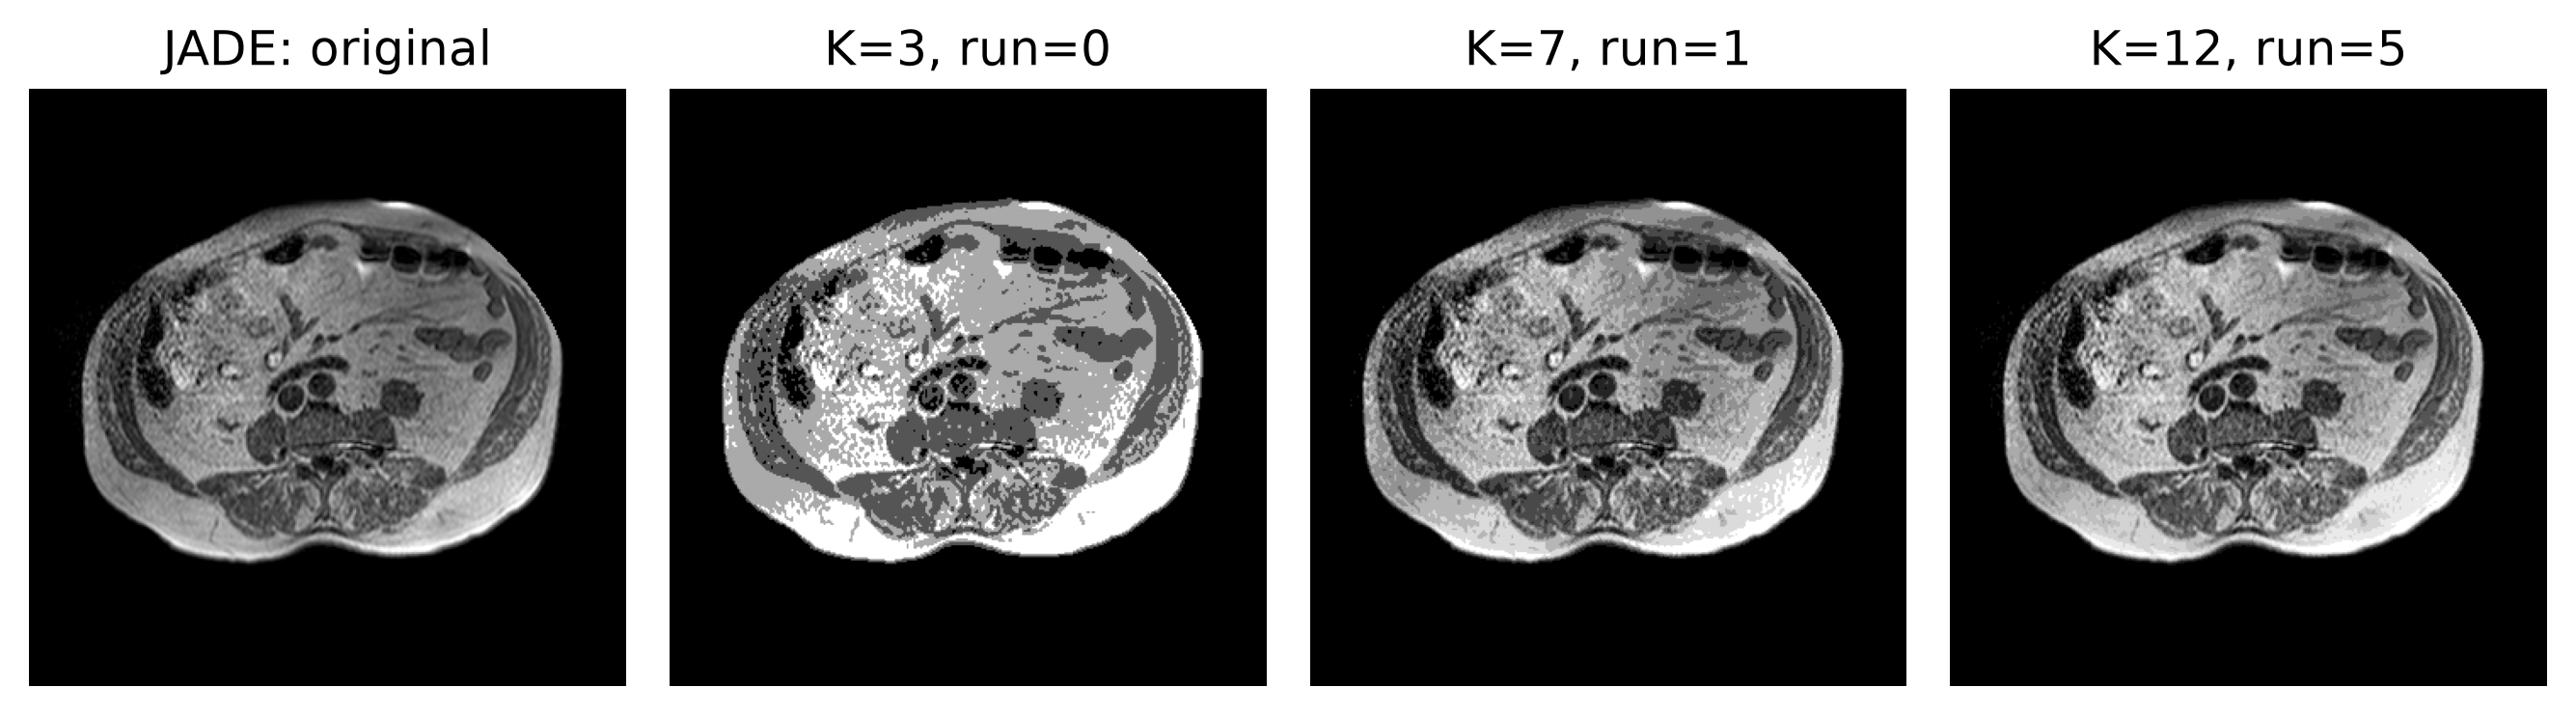
\includegraphics[width=0.9\textwidth]{exp2_segmentation_otsu.png}
\caption{Original and thresholded image IMG-0003-00010 using Otsu at $K=3,7,12$. Rows: JADE. Solutions are selected by final fitness closest to the median, with ties resolved by the lowest run index. The displayed run number identifies an independent repetition.}
\label{fig:chaos-otsu}
\end{figure}

\begin{figure}[htbp]
\centering
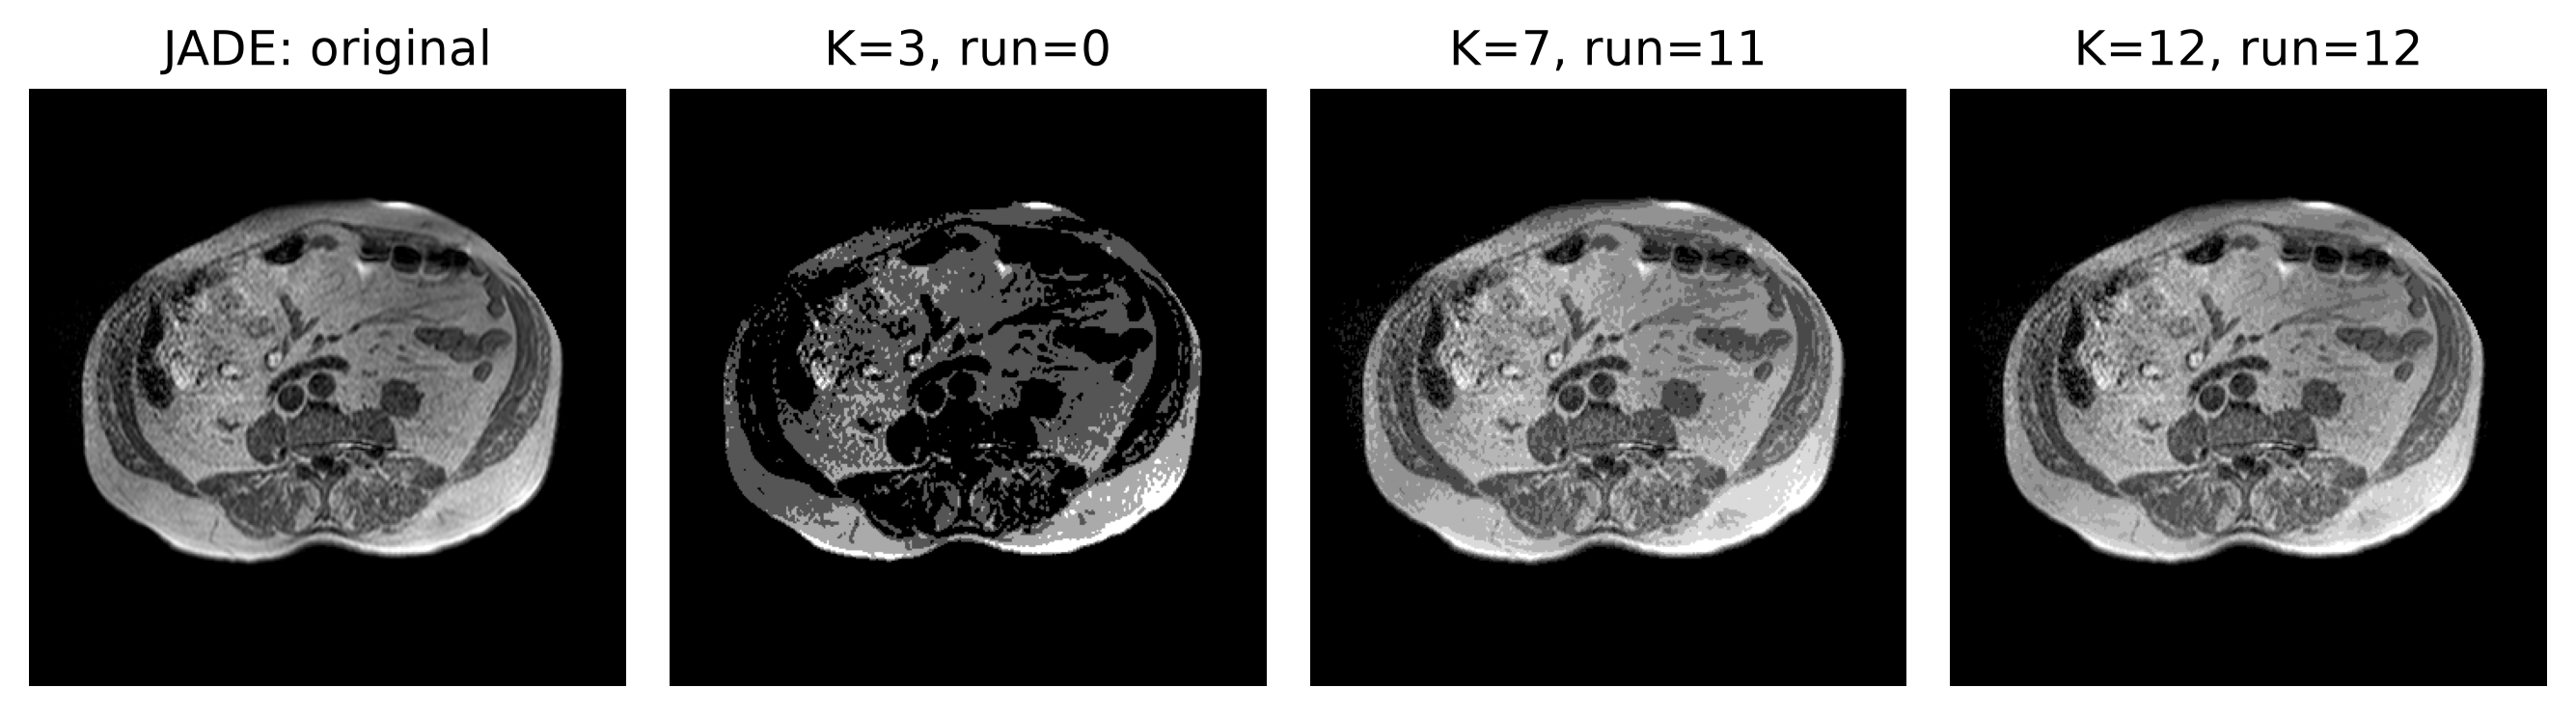
\includegraphics[width=0.9\textwidth]{exp2_segmentation_kapur.png}
\caption{Original and thresholded image IMG-0003-00010 using Kapur at $K=3,7,12$. Rows: JADE. Solutions are selected by final fitness closest to the median, with ties resolved by the lowest run index. The displayed run number identifies an independent repetition.}
\label{fig:chaos-kapur}
\end{figure}

\begin{figure}[htbp]
\centering
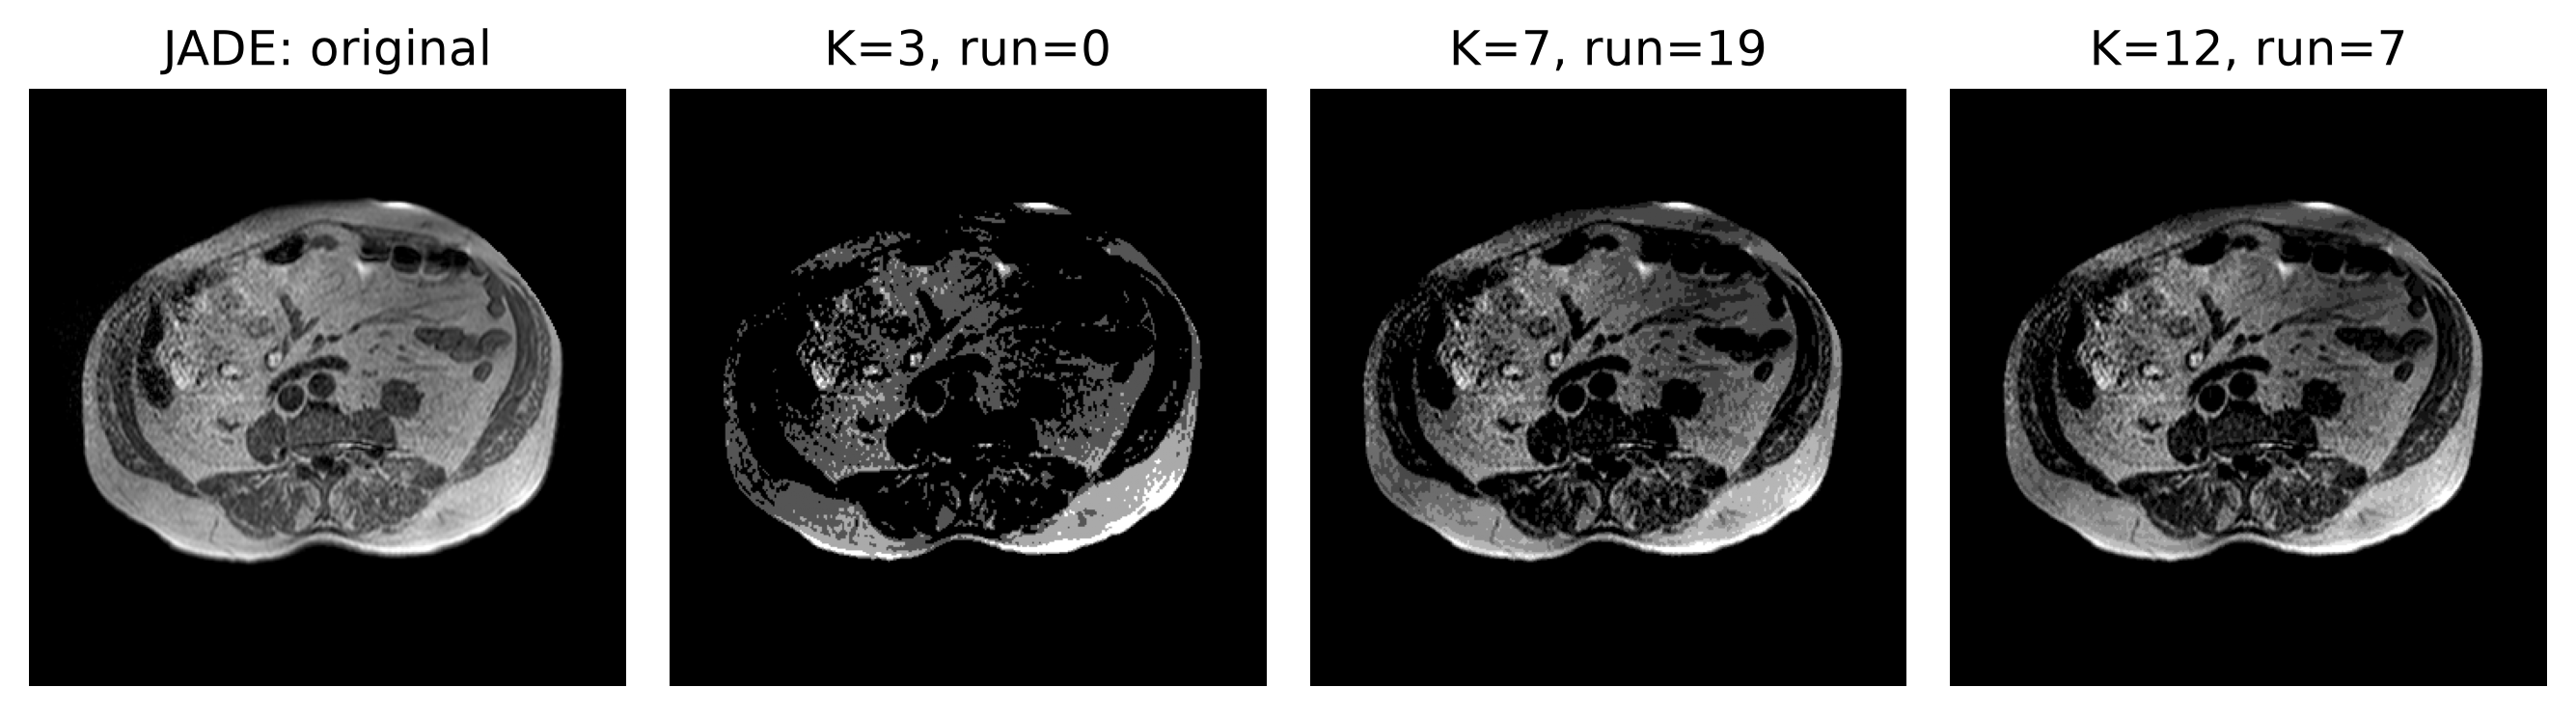
\includegraphics[width=0.9\textwidth]{exp2_segmentation_tsallis.png}
\caption{Original and thresholded image IMG-0003-00010 using Tsallis at $K=3,7,12$. Rows: JADE. Solutions are selected by final fitness closest to the median, with ties resolved by the lowest run index. The displayed run number identifies an independent repetition.}
\label{fig:chaos-tsallis}
\end{figure}

\subsection{Convergence Analysis}

\begin{figure}[htbp]
\centering
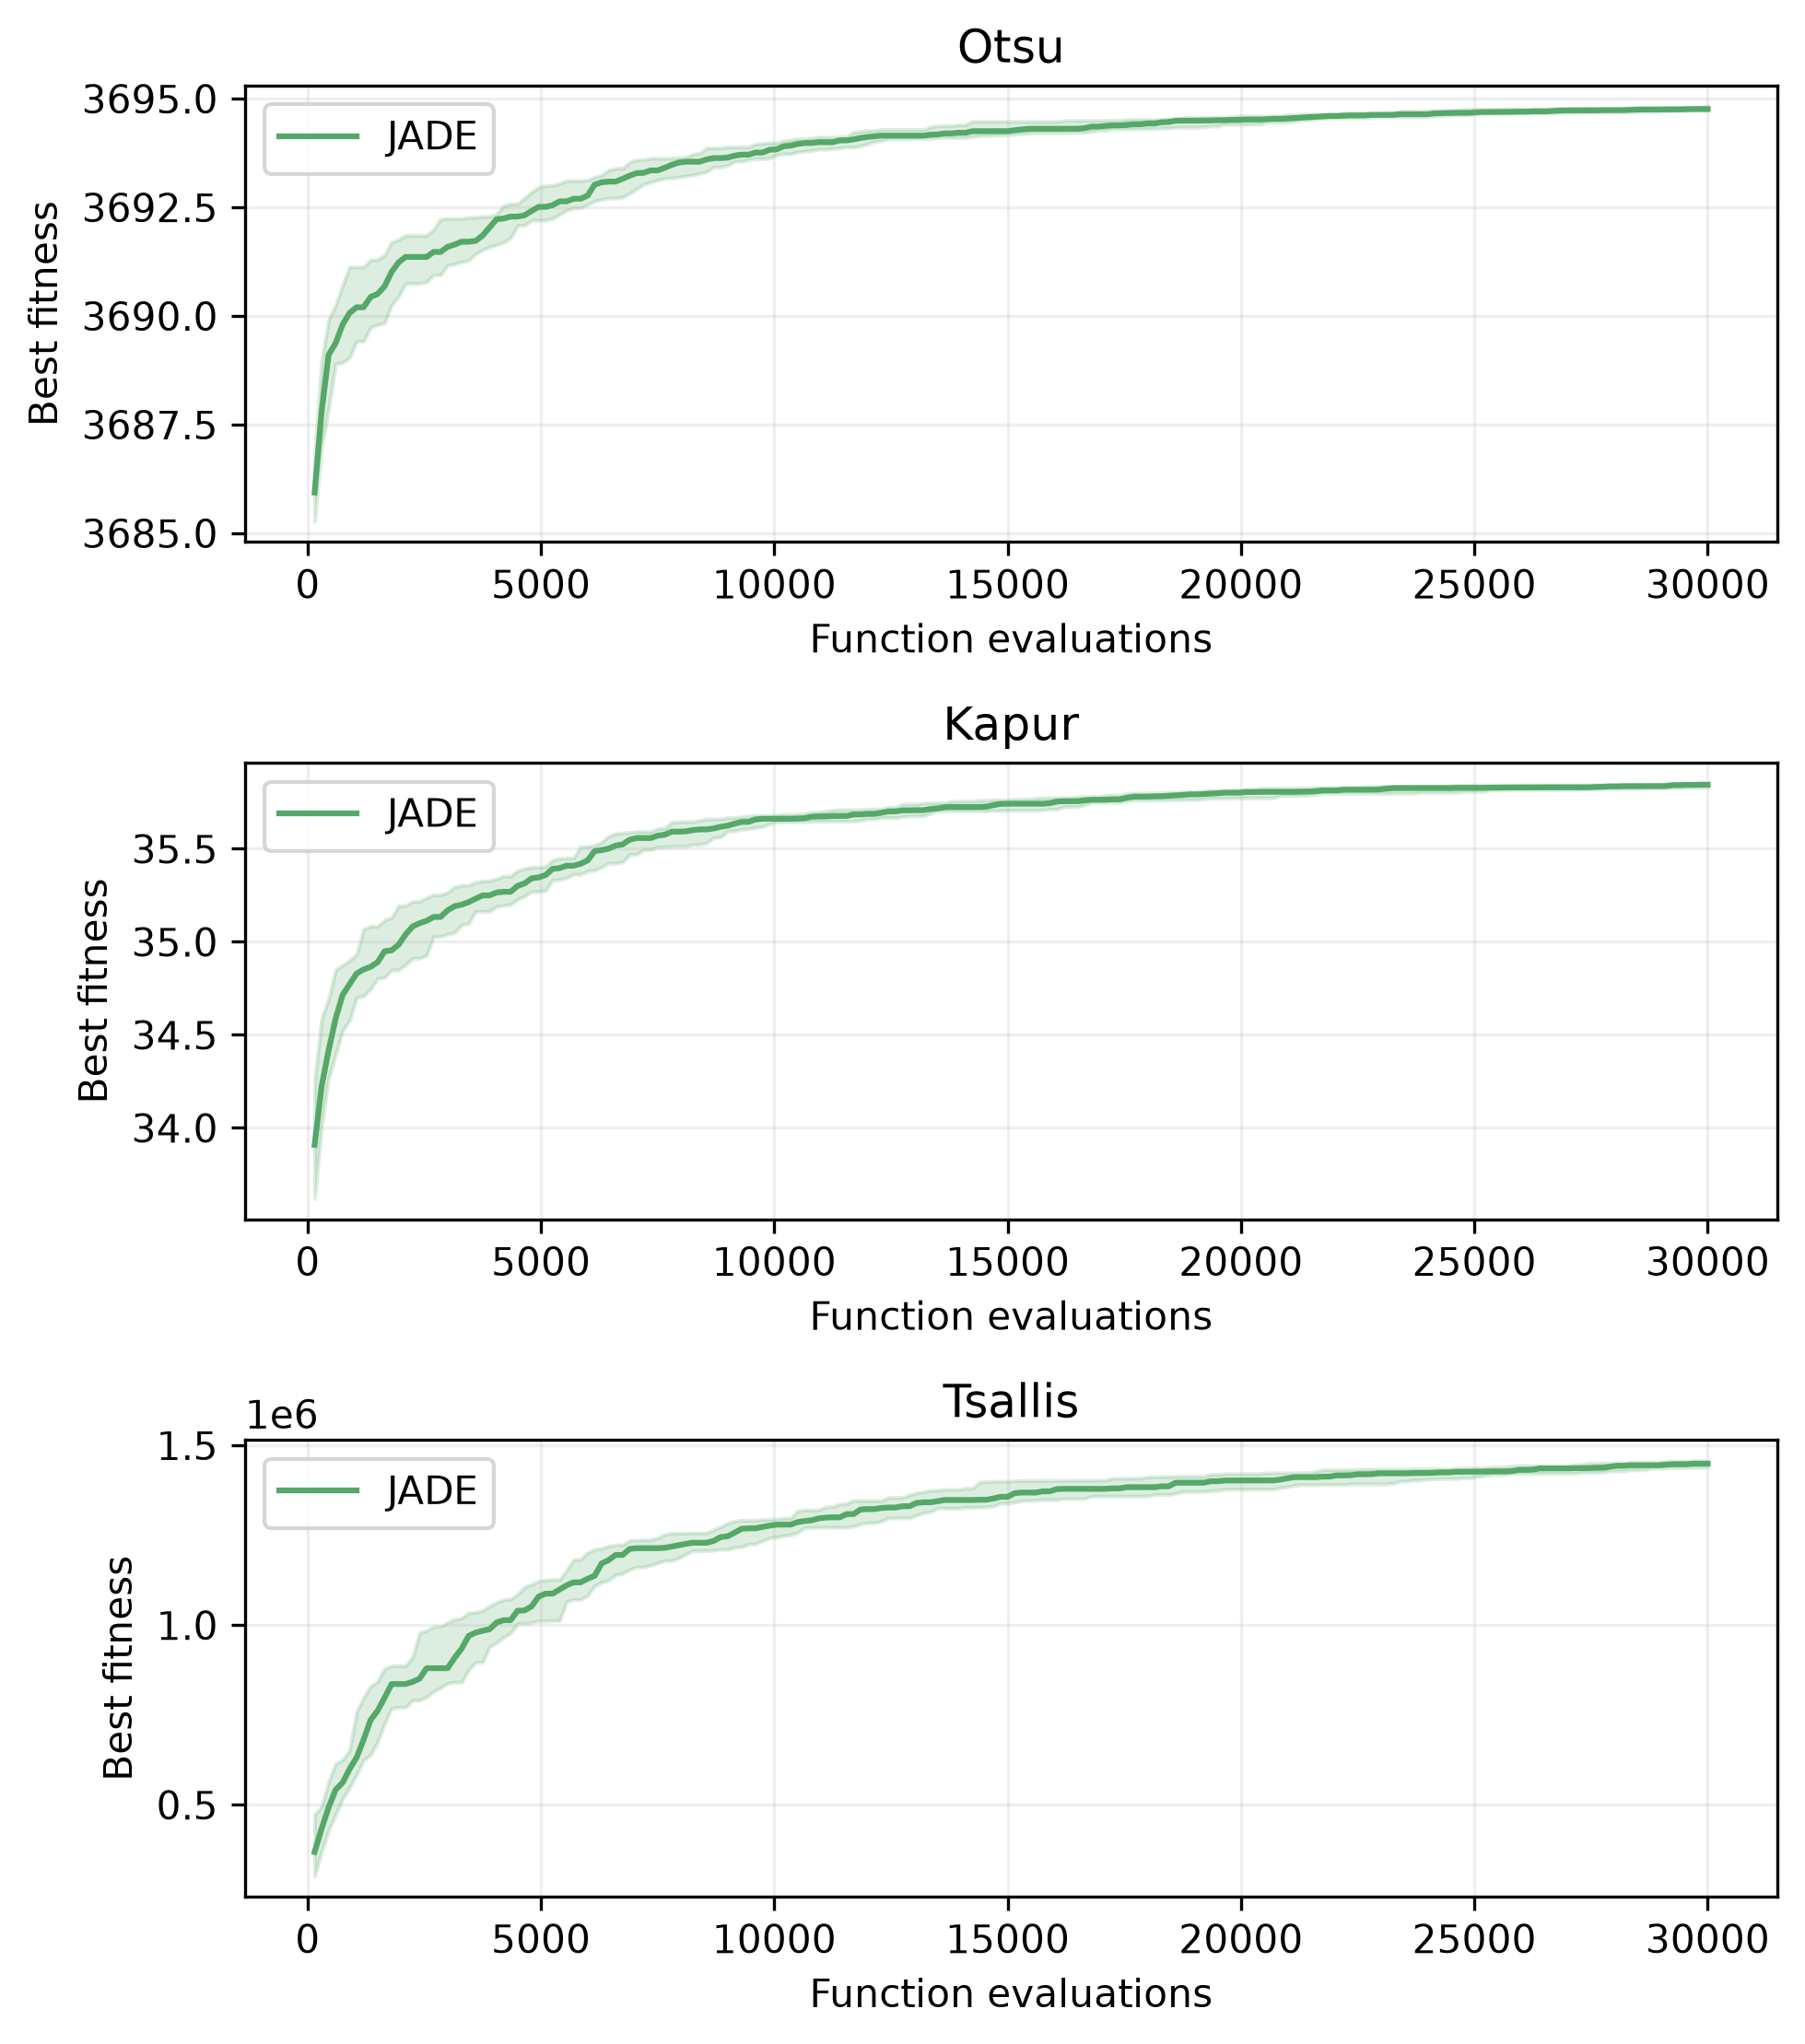
\includegraphics[width=0.9\textwidth]{exp2_convergence.png}
\caption{Best-so-far fitness for image IMG-0003-00010 at $K=12$. Lines show medians over 30 runs; bands show interquartile ranges.}
\label{fig:chaos-convergence}
\end{figure}

\subsection{Execution Time}

\begin{figure}[htbp]
\centering
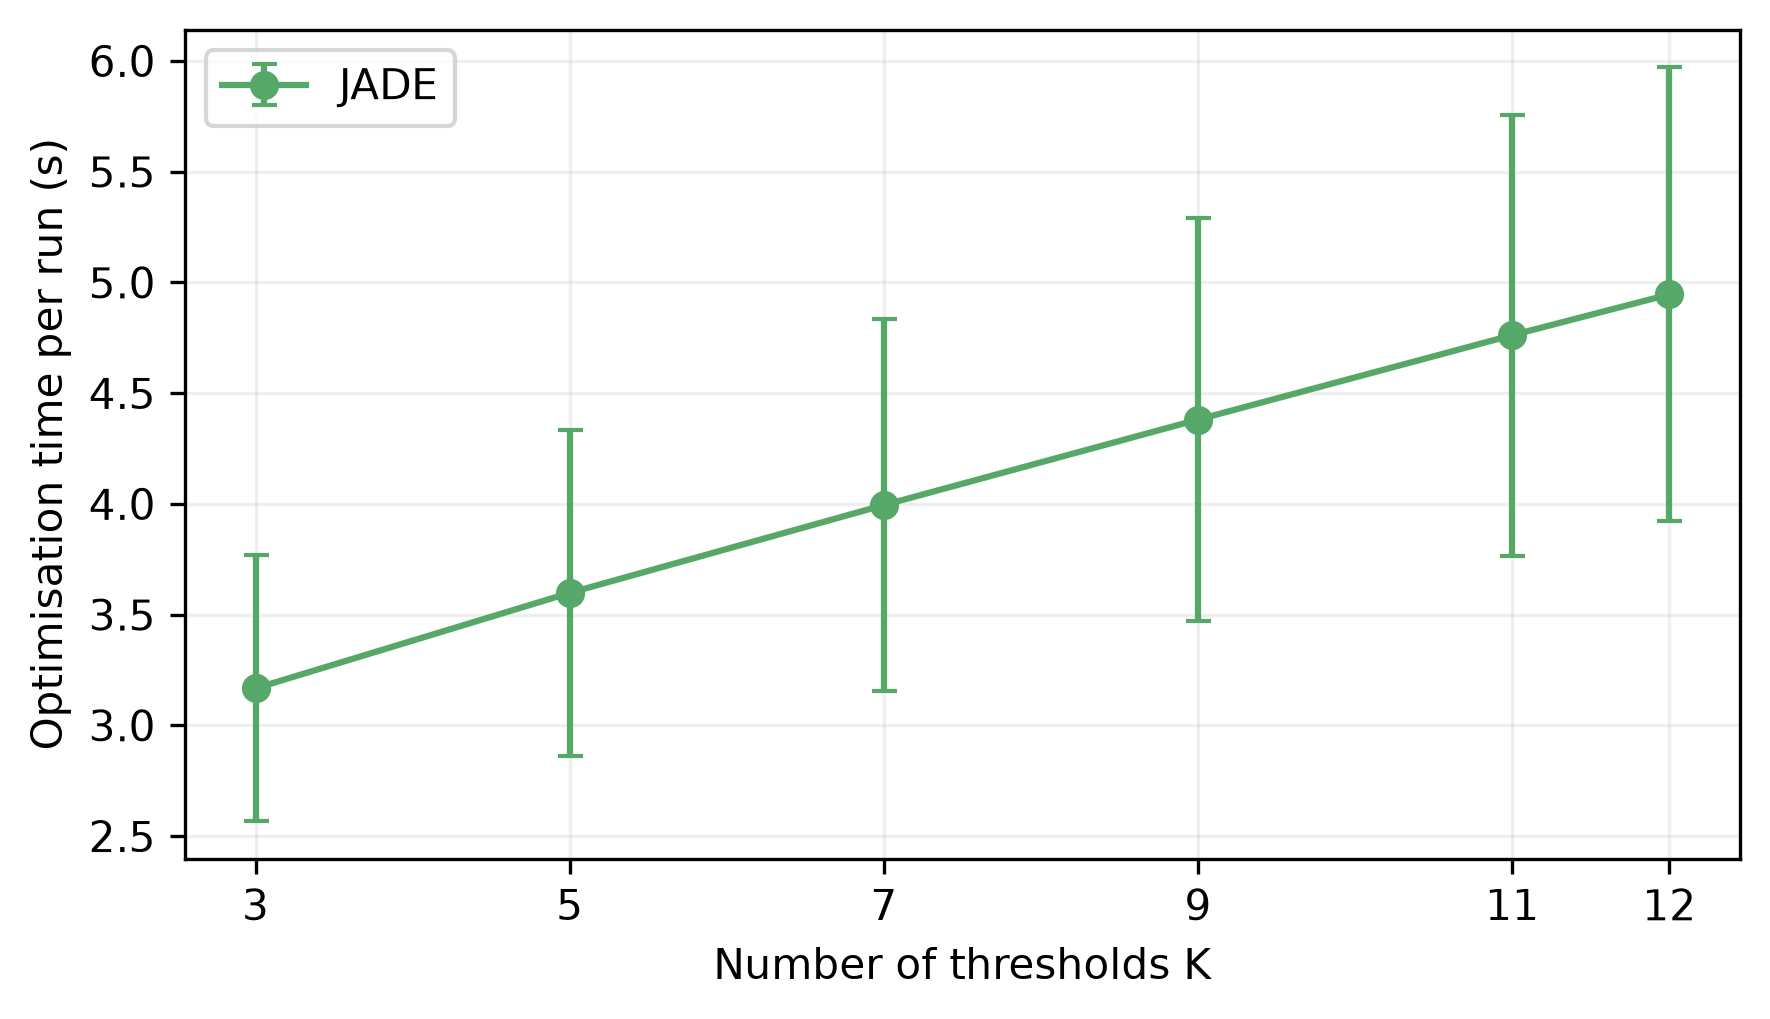
\includegraphics[width=0.9\textwidth]{exp2_runtime.png}
\caption{Mean recorded optimisation time versus $K$, with sample standard deviation as error bars, pooled across images, objectives and runs.}
\label{fig:chaos-runtime}
\end{figure}

\subsection{Discussion of Experiment 2}

--

\section{Statistical Analysis}
\label{sec:statistics}

Because stochastic evolutionary algorithms may produce different
solutions across independent runs, statistical tests are used to
determine whether observed performance differences are statistically
significant.

A significance level of

\begin{equation}
\alpha = 0.05
\end{equation}

is used.


\subsection{Wilcoxon Signed-Rank Test}

% If using Wilcoxon:
%
% Clearly state:
% - paired observations being compared
% - H0
% - H1
% - significance level
% - multiple-comparison handling if used
%
% DO NOT just report p-values without interpretation.


\subsection{Friedman Test}

% If using Friedman:
%
% Explain:
% - datasets/tasks as blocks
% - algorithms as treatments
% - H0: equivalent algorithm ranks
% - significance decision
% - post-hoc testing if performed


\begin{table}[H]
\caption{Statistical comparison of optimisation algorithms.}
\label{tab:stats}
\centering

\begin{tabular}{llll}
\toprule
Comparison & Metric & $p$-value & Significant? \\
\midrule

DE vs JADE      & -- & -- & -- \\
DE vs SHADE     & -- & -- & -- \\
DE vs L-SHADE   & -- & -- & -- \\
DE vs LADE      & -- & -- & -- \\

\bottomrule
\end{tabular}

\end{table}


% =========================================================
% 9. SCALABILITY AND COMPUTATIONAL ANALYSIS
% =========================================================

\section{Computational Scalability Analysis}
\label{sec:scalability}


\subsection{Execution Time versus Number of Thresholds}

\begin{figure}[H]
    \centering
    % \includegraphics[width=0.8\textwidth]{runtime_vs_k.pdf}
    \caption{Mean execution time as a function of threshold level $K$.}
    \label{fig:runtime}
\end{figure}

% Discuss:
%
% Does runtime increase with K?
% Linear/non-linear?
% Algorithm differences?
% Impact of adaptation/archive/history?
% Does L-SHADE's population reduction affect runtime?


\subsection{Convergence Rate}

% Compare the number of FEs required to reach a given quality,
% or directly compare convergence curves.


\subsection{Impact of Increasing Dimensionality}

% Important discussion:
%
% Search vector dimension == K.
%
% K=3 => 3-dimensional optimisation problem
% K=12 => 12-dimensional optimisation problem
%
% Explain:
% - search-space growth
% - convergence difficulty
% - variability
% - population diversity
% - premature convergence if observed


% =========================================================
% 10. DISCUSSION
% =========================================================

\section{Discussion}
\label{sec:discussion}

% This is one of the most important report sections.
%
% Don't simply repeat Results.
%
% Suggested structure:


\subsection{Comparison of Differential Evolution Variants}

% Compare the mechanisms behind observed behaviour.
%
% Standard DE:
% fixed F/CR, baseline
%
% JADE:
% parameter adaptation + p-best
%
% SHADE:
% successful parameter history
%
% L-SHADE:
% success-history + population reduction
%
% LADE:
% late acceptance behaviour


\subsection{Impact of Objective Function}

% Compare Otsu/Kapur/Tsallis across both datasets.


\subsection{Impact of Tsallis Non-Extensivity Parameter}

% Assignment specifically asks for critical analysis of q.
%
% Discuss what q does and what you observed empirically.


\subsection{BSD500 versus CHAOS MRI}

% Compare:
% - generic image segmentation
% - medical image segmentation
% - intensity distributions
% - stability
% - GT-based metrics


\subsection{Algorithm Robustness}

% Use standard deviation, statistical testing, and convergence
% evidence rather than only best-run performance.


\subsection{Limitations}

Possible limitations include:

\begin{itemize}
    \item evaluation on a limited number of images;
    \item dependence on selected DE parameter settings;
    \item use of a fixed Tsallis $q$ value, if applicable;
    \item stochastic variability between runs;
    \item computational cost associated with repeated optimisation; and
    \item limitations of intensity-only thresholding for complex
          anatomical structures.
\end{itemize}


% =========================================================
% 11. CONCLUSION
% =========================================================

\section{Conclusion}
\label{sec:conclusion}

This study evaluated five Differential Evolution algorithms for
multilevel image thresholding using Otsu, Kapur, and Tsallis objective
functions across six threshold dimensions.

% AFTER RESULTS, answer:
%
% - What did you learn?
% - How did adaptive algorithms behave relative to baseline DE?
% - What happened as K increased?
% - What happened on BSD500 vs CHAOS?
% - What was the impact of objective-function selection?
% - What did statistical analysis establish?
%
% Avoid introducing new results here.


% =========================================================
% OPTIONAL FUTURE WORK
% =========================================================

\section{Future Work}

Possible extensions include evaluation on larger medical imaging
datasets, adaptive optimisation of the Tsallis $q$ parameter, alternative
population adaptation strategies, and hybridisation with other
metaheuristic optimisation techniques.


% =========================================================
% AUTHOR CONTRIBUTIONS
% =========================================================

\section*{CRediT authorship contribution statement}

\textbf{Aryan Mohanlall:}
% Replace with actual responsibilities.
Standard DE and Late Acceptance DE implementation.

\textbf{Second Author:}
% Insert actual contributions.

\textbf{Third Author:}
% Insert actual contributions.

\textbf{Fourth Author:}
% Insert actual contributions.


% =========================================================
% DECLARATIONS
% =========================================================

\section*{Declaration of Competing Interest}

The authors declare that they have no known competing financial
interests or personal relationships that could have appeared to
influence the work reported in this paper.


\section*{Acknowledgements}

% Add acknowledgements only if appropriate.


\section*{Data availability}

The source code, experimental configurations, and generated results
used in this study are provided in the accompanying assignment
submission repository.

% Replace with repository URL if required.


% =========================================================
% REFERENCES
% =========================================================

\bibliographystyle{ieeetr}
\bibliography{references}

\end{document}
